%%::::::::::::::::::::::::::::::::::::::::::::::::::::::::::::::::::::::::::::::
%%
%%    This file is part of ICTP RegCM.
%%    
%%    Use of this source code is governed by an MIT-style license that can
%%    be found in the LICENSE file or at
%%
%%         https://opensource.org/licenses/MIT.
%%
%%    ICTP RegCM is distributed in the hope that it will be useful,
%%    but WITHOUT ANY WARRANTY; without even the implied warranty of
%%    MERCHANTABILITY or FITNESS FOR A PARTICULAR PURPOSE.
%%
%%::::::::::::::::::::::::::::::::::::::::::::::::::::::::::::::::::::::::::::::

\newpage

\chapter{Model Equations}

The \ac{RegCM} model solves a set of primitive dynamical equations describing
the atmospheric motion, with parametrizations for physical processes as per:

\begin{itemize}
  \item Radiation (Short Wave and Long Wave)
  \item Convection
  \item Turbulent Diffusion
  \item Moist (Clouds and Precipitation)
  \item Fluxes exchange with surface (Soil model and Ocean fluxes)
  \item Tracer transport and chemistry (Aerosols and full chemistry)
\end{itemize}

The dynamical equations are discretized using finite differences technique
on a three dimensional computation grid with fixed horizontal resolution
and terrain following vertical coordinate.

\section{Dynamics}
The model has three dynamical cores:

\begin{itemize}
\item Hydrostatic equation solver
\item Non-hydrostatic equation solver with pressure coordinate
\item Non-hydrostatic equation solver with height coordinate
\end{itemize}

The primitive equations for the three solvers are different and have different
prognostic variables used to identify the atmospheric state.

\subsection{Hydrostatic dynamical core}
The hydrostatic model dynamic equations and numerical discretization are
described by \cite{Grell_94}.

\subsubsection{Horizontal Momentum Equations}

\begin{gather}
\label{hydro_mom1}
  \frac{\partial{p^{\ast}u}}{\partial{t}} =
  -m^2 \left[ \frac{\partial{p^{\ast}uu/m}}{\partial{x}} + 
    \frac{\partial{p^{\ast}vu/m}}{\partial{y}} \right] -
    \frac{\partial{p^{\ast}u \dot{\sigma}}}{\partial{\sigma}}
      \\ \nonumber
      -mp^{\ast} \left[ \frac{\sigma}{\rho}
      \frac{\partial{p^{\ast}}}{\partial{x}} +
      \frac{\partial{\phi}}{\partial{x}} \right] +
  p^{\ast}fv + F_Hu + F_Vu \\
\label{hydro_mom2}
  \frac{\partial{p^{\ast}v}}{\partial{t}} = 
  -m^2 \left[ \frac{\partial{p^{\ast}uv/m}}{\partial{x}} +
    \frac{\partial{p^{\ast}vv/m}}{\partial{y}} \right] -
    \frac{\partial{p^{\ast}v\dot{\sigma}}}{\partial{\sigma}}
     \\ \nonumber
     -mp^{\ast} \left[ \frac{\sigma}{\rho}
         \frac{\partial{p^{\ast}}}{\partial{y}} +
      \frac{\partial{\phi}}{\partial{y}} \right]
  + p^{\ast}fu + F_Hv + F_Vv
\end{gather}

where $u$ and $v$ are the eastward and northward components of
velocity, $\phi$ is geopotential height, $f$ is the Coriolis parameter,
$m$ is the map scale factor for the chosen projection, and $F_H$ and $F_V$
represent the effects of horizontal and vertical diffusion, and
$p^{\ast} = p_s-p_t$, i.e. the difference between surface and model top
pressure.  \\

In the equation \ref{hydro_mom1} - \ref{hydro_mom2}, $\dot{\sigma}$ is the total
derivative of the vertical coordinate $\sigma$ over time $t$:

\begin{equation}
\dot{\sigma} = {d\sigma \over dt}
\end{equation}

Moreover, given $T_v$ as the virtual temperature:

\begin{equation}
T_v = T \left( 1 + 0.608 Q_v \right)
\end{equation}

then

\begin{equation}
\frac{\sigma}{\rho} = \frac{RT_v}{(p^{\ast} + p_t/\sigma)}
\end{equation}

with $R$ the gas constant for dry air

\subsubsection{Continuity and Sigmadot $({\bf \dot{\sigma}})$ Equations}

The surface pressure is computed from the continuity equation:

\begin{eqnarray} \label{eq:continuity}
\frac{\partial{p^{\ast}}}{\partial{t}} = 
  -m^2 \left[ \frac{\partial{p^{\ast}u/m}}{\partial{x}} +
        \frac{\partial{p^{\ast}v/m}}{\partial{y}} \right] -
  \frac{\partial{p^{\ast}\dot{\sigma}}}{\partial{\sigma}}
\end{eqnarray}

The vertical integral of Equation~\ref{eq:continuity} is used to
compute the temporal variation of the surface pressure in the model,

\begin{eqnarray}
\label{intform}
  \frac{\partial{p^{\ast}}}{\partial{t}} = -m^2 \int_{0}^{1}
  {\left[ \frac{\partial{p^{\ast}u/m}}{\partial{x}} + 
    \frac{\partial{p^{\ast}v/m}}{\partial{y}} \right] d\sigma}
\end{eqnarray}

The surface pressure tendency from \ref{intform} is then used with
the vertical integral of \ref{eq:continuity} to compute the vertical
velocity in sigma coordinates $(\dot{\sigma})$ at each
level in the model:

\begin{eqnarray}
  \dot{\sigma} = - \frac{1}{p^{\ast}} \int_{0}^{\sigma}{
    \left[ \frac{\partial{p^{\ast}}}{\partial{t}} +
    m^2 \left(\frac{\partial{p^{\ast}u/m}}{\partial{x}} +
                     \frac{\partial{p^{\ast}v/m}}{\partial{y}}
   \right) \right] d\sigma^\prime}
\end{eqnarray}

where $\sigma^\prime$ is a dummy variable of integration and
$\dot{\sigma}(\sigma=0)=0$, $\dot{\sigma}(\sigma=1)= 0$.

\subsubsection{Thermodynamic Equation and Equation for Omega ${\bf (\omega)}$}

The thermodynamic equation is

\begin{eqnarray}
\frac{\partial{p^{\ast}T}}{\partial{t}} = 
-m^2 \left[ \frac{\partial{p^{\ast}uT/m}}{\partial{x}} +
      \frac{\partial{p^{\ast}vT/m}}{\partial{y}} \right] -
      \frac{\partial{p^{\ast}T\dot{\sigma}}}{\partial{\sigma}} +
      \nonumber \\
  \frac{RT_v\omega}{c_{p}(\sigma + p_t/p_{\ast})} +
  \frac{p^{\ast}Q}{c_{p}} + F_HT + F_VT
\end{eqnarray}

where, given $c_{pd}$ the heat capacity of dry air and
$q_v$ the water vapor mixing ratio:

\begin{equation}
c_{p} = c_{pd} \left( 1 + 0.8q_v \right)
\end{equation}

$c_p$ is the specific heat for moist air at constant pressure, $Q$ is the
diabatic heating, $F_HT$ represents the effect of horizontal diffusion,
$F_VT$ represents the effect of vertical mixing and dry convective adjustment,
and $\omega$ is

\begin{equation}
  \omega = \frac{dp}{dt} = p^{\ast} \dot{\sigma} +
            \sigma \frac{dp^{\ast}}{dt}
\end{equation}

where:
  
\begin{eqnarray}
\frac{dp^{\ast}}{dt} =
   \frac{\partial{p^{\ast}}}{\partial{t}} + m
   \left[ u \frac{\partial{p^{\ast}}}{\partial{x}} +
          v \frac{\partial{p^{\ast}}}{\partial{y}} \right]
\end{eqnarray}

\subsubsection{Hydrostatic Equation}

The hydrostatic equation is used to compute the geopotential heights from
the virtual temperature $T_v$,

\begin{eqnarray}
\label{hydrostatic_equation}
\frac{\partial{\phi}}{\partial{\ln(\sigma + p_t / p^{\ast})}} =
-RT_v \left[ 1 + \frac{\sum{q_x}}{1 + q_v} \right]^{-1}
\end{eqnarray}

where $T_v = T(1 + 0.608q_v)$, $q_v$, is the water vapor mixing ratio, and
$q_x$ are the mixing ratios of all condensed water species.

\subsubsection{Horizontal advection equation discretization}

\begin{figure}
\begin{center}
\resizebox{4.0in}{!}{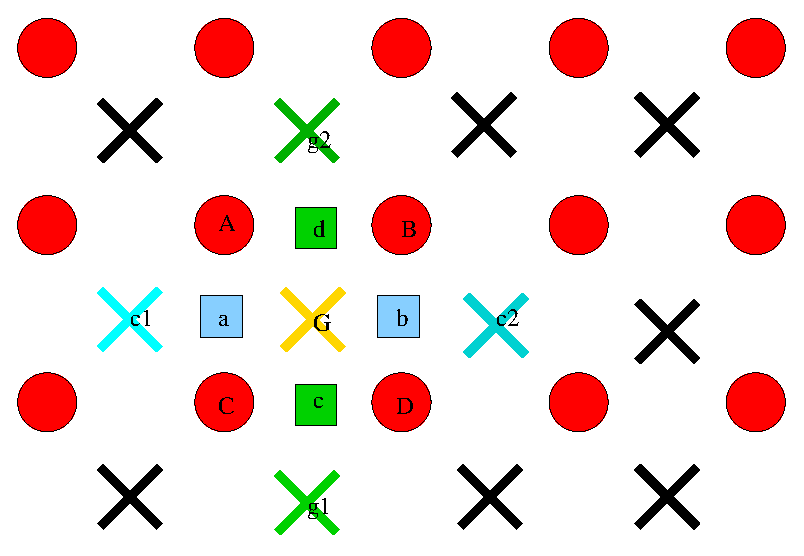
\includegraphics{advection.eps}}
\caption{Schematic representation showing the horizontal advection
scheme staggering. Circles are U,V points. X are scalar variable points.}
\label{advection_grid}
\end{center}
\end{figure}

The advection equation for the generic scalar variable contributes to the total
timestep tendency for the variable with a term :

\begin{eqnarray}
\label{advection_equation_1}
\Delta_{adv} \left(p^* X\right)_{G} = -m^2|_G \left[ 
  \frac{\left( p^*X|_b \frac{u}{m}|_b-p^*X|_a \frac{u}{m}|_a \right)}{dx} +
  \frac{\left( p^*X|_d \frac{v}{m}|_d-p^*X|_c \frac{v}{m}|_c \right)}{dy}\right]
\end{eqnarray}

With reference to figure \ref{advection_grid}, assuming the computation
is to be performed for the gold cross point $G$, the averages are performed in
points $a,b,c,d$.
For the $u/m$ and $v/m$ terms, the average value is computed using respectively
the values in points $AC,BD,CD,AB$.
For the term $p^*X$, the model computes a weighted average value of the field
using the value in gold+cyan and gold+green cross points with weights
increasing the relative contribution of the upstream point up to a maximum
configurable factor function of the local courant number:

\begin{eqnarray}
\label{advection_equation_2}
p^*X|_a = 0.5 ( (1-f_1) p^*X|_{G} + (1+f_1) p^*X|_{c_1} ) \\
p^*X|_b = 0.5 ( (1-f_1) p^*X|_{c_2} + (1+f_1) p^*X|_{G} ) \\
p^*X|_c = 0.5 ( (1-f_2) p^*X|_{G} + (1+f_2) p^*X|_{g_1} ) \\
p^*X|_d = 0.5 ( (1-f_2) p^*X|_{g_2} + (1+f_2) p^*X|_{G} )
\end{eqnarray}

where $f_1,f_2$ are defined as the local Courant number for the 1D advection
equations multiplied for a control factor:

\begin{eqnarray}
\label{advection_equation_3}
f_1 = \mu_{fc} dt \frac{(u|_a + u|_b)}{2dx} \\
f_2 = \mu_{fc} dt \frac{(v|_c + v|_d)}{2dy}
\end{eqnarray}

being $dt$ the model timestep in seconds, $dx,dy$ the grid sizes in meters and
$\mu_{fc}$ a namelist configurable parameter. The $f_1,f_2$ can be set
to zero by disabling in the namelist the horizontal advection upstream mode.

The wind components horizontal advection term requires triple averaging in
the horizontal momentum advection terms, and it is described in
\cite{Anthes_72}.

\subsubsection{Split-explicit timestep for fast waves removal}

The vertical modes initialization is  described in \cite{Errico_88}.

The hydrostatic model equations above (\ref{hydro_mom1}-
\ref{hydrostatic_equation}) can be linearized about a state at rest,
with:

\begin{gather}
\label{reference_atm}
  \mean{u} = 0 \nonumber \\
  \mean{v} = 0 \nonumber \\
  T = \mean{T} \nonumber \\
  f_0 = \mean{f} \nonumber \\
  p^{\ast} = \mean{p}
\end{gather}

The linearized equations are:

\begin{gather}
  \label{linearized}
  \frac{\partial u}{\partial t} =
       f_0 v - \frac{\partial}{\partial x} (\phi^{\prime} +
       R\mean{T}\ln^{\prime}(\sigma p^{\ast} + p_t)) \\
  \frac{\partial v}{\partial t} =
       - f_0 u - \frac{\partial}{\partial y} (\phi^{\prime} +
       R\mean{T}\ln^{\prime}(\sigma p^{\ast} + p_t)) \\
  \frac{\partial T^\prime}{\partial t} =
     - \dot{\sigma} \frac{\partial \mean{T}}{\partial \sigma} +
     \frac{\kappa \mean{T}}{\sigma + \frac{p_t}{\mean{p}}}
     \frac{\omega}{\mean{p}} \\
  \label{2111a}
  \frac{\partial \ln\left(\frac{p^{\ast}}{\mean{p}}\right)}{\partial t} =
  -\int_0^1\left(\frac{\partial u}{\partial x} +
  \frac{\partial v}{\partial y} \right) d\sigma \\
  \label{2111b}
  \frac{\partial}{\partial t} \ln^{\prime}\left(\sigma p^{\ast} +
     p_t\right) = \frac{\sigma}{\sigma+\frac{p_t}{\mean{p}}}
        \frac{\partial}{\partial t}
        \ln\left(\frac{p^{\ast}}{\mean{p}}\right) \\
  \phi^{\prime} = \phi_S - R \int_0^1 T^{\prime}
    d \left[ \ln(\sigma \mean{p}+p_t)\right] -
    R \int_0^1 \mean{T} d \left[ \ln^{\prime}
    (\sigma p^{\ast}+p_t) \right] \\
  \dot{\sigma} = \sigma \int_0^1 \left(\frac{\partial u}{\partial x} +
  \frac{\partial v}{\partial y} \right) d\sigma -
  \int_0^{\sigma} \left(\frac{\partial u}{\partial x} +
  \frac{\partial v}{\partial y}\right) d\sigma^{\prime} \\
  \label{last_linearized}
  \frac{\omega}{\mean{p}} = \dot{\sigma} - \sigma
  \int_0^1 \left(\frac{\partial u}{\partial x} +
  \frac{\partial v}{\partial y}\right) d\sigma
\end{gather}

where

\begin{gather}
  T^{\prime}(x,y,t,\sigma) = T(x,y,t,\sigma) -
     \mean{T}(\sigma) \nonumber \\
  \ln^{\prime}(\sigma p^{\ast} + p_t) = \ln(\sigma p^{\ast} + p_t) -
    \ln(\sigma \mean{p} + p_t) \nonumber \\
  \kappa = \frac{R}{c_p} \nonumber
\end{gather}

Substituting now coordinates $u,v$ with horizontal vorticity $\zeta$ and
divergence $\delta$ defined as:

\begin{gather}
  \label{vorticity}
  \zeta = \frac{\partial v}{\partial x} -
          \frac{\partial u}{\partial y} \\
  \label{divergence}
        \delta = \frac{\partial u}{\partial x} +
                 \frac{\partial v}{\partial y}
\end{gather}

and defining the stream function $\psi$ and the velocity potential $\chi$
by:

\begin{gather}
  \left(\frac{\partial^2}{\partial x^2} +
        \frac{\partial^2}{\partial y^2}\right) \psi = 
        \nabla^2 \psi = \zeta \\
  \left(\frac{\partial^2}{\partial x^2} +
        \frac{\partial^2}{\partial y^2}\right) \chi = 
        \nabla ^2 \chi = \delta \\
  u = \frac{\partial \chi}{\partial x} -
      \frac{\partial \psi}{\partial y} \\
  v = \frac{\partial \chi}{\partial y} +
      \frac{\partial \psi}{\partial x}
\end{gather}

we obtain:

\begin{gather}
  \frac{\partial \zeta}{\partial t} = -f_0 \delta \\
  \frac{\partial \delta}{\partial t} = f_0 \zeta -
    \nabla^2\left[\phi^{\prime} + R \mean{T}
    \ln^{\prime}\left(\sigma p^{\ast} + p_t\right)\right] \\
  \label{2124}
  \frac{\partial T^{\prime}}{\partial t} = \bm{A} \delta \\
  \label{2125}
  \phi^{\prime} = \phi_S + R \bm{B} T^{\prime} +
      R \bm{C} \ln^{\prime} \left(\sigma p^{\ast} + p_t\right)
\end{gather}

where $\bm{A}, \bm{B}, \bm{C}$ are integral-differential operators in $\sigma$
function of $\mean{T}$ and $\frac{p_t}{\mean{p}}$.

Defining now the pseudo-geopotential $h$ as:

\begin{gather}
  \label{pseudogeop}
  h = \phi^{\prime} + R \mean{T} \ln^{\prime}
      \left(\sigma p^{\ast} + p_t\right)
\end{gather}

combining \ref{2125}, \ref{2124} and \ref{2111a}, we can derive time tendency
of this pseudo-geopotential $h$ as:

\begin{gather}
  \frac{\partial h}{\partial t} = - \tau(\delta)
\end{gather}

with $\tau$ is the integral $\sigma$-coordinate operator:

\begin{gather}
  \tau( ) = -R \bm{B}\bm{A}( ) + R \left( \bm{C} + \mean{T} \right)
    \frac{\sigma}{\sigma + \frac{p_t}{\mean{p}}}
    \int_0^1 ( ) d\sigma
\end{gather}

The complete nonlinear equations may be written as:

\begin{gather}
  \label{cmplnonlin1}
  \frac{\partial \zeta}{\partial t} = -f_0 \delta + N_{\zeta} \\
  \label{cmplnonlin2}
  \frac{\partial \delta}{\partial t} = f_0 \zeta -
     \nabla^2 h + N_{\delta} \\
  \label{cmplnonlin3}
  \frac{\partial h}{\partial t} = - \tau(\delta) + N_{h} \\
  \frac{\partial p^{\ast}}{\partial t} = -
     \int_0^1 \left(\frac{\partial p^{\ast}u}{\partial x} +
     \frac{\partial p^{\ast} v}{\partial y} \right) d\sigma
\end{gather}

where the non linear terms contains also horizontal variations of $f$.

If we now impose the conditions:

\begin{itemize}
  \item the primitive equations have slow behavior
  \item the time tendencies of the amplitudes of gravitational waves are
    negligible compared with other terms in the prognostic equations
  \item the linearized potential vorticity
    $\eta = \zeta - f_0 \tau^{-1}(h)$ is unchanged
\end{itemize}

we have:

\begin{gather}
  f_0 \zeta - \nabla^2 h = -N_{\delta} \\
  \frac{\partial}{\partial t}\left( f_0 \zeta - \nabla^2 h\right) = 0 \\
  \frac{\partial \eta}{\partial t} = 
   \frac{\partial \left(\zeta - f_0 \tau^{-1}(h)\right)}{\partial t} = 0
\end{gather}

The complete set of equations for the balance condition is:

\begin{gather}
  \label{balance_condition_1}
  \left(f_0^2 \tau^{-1} - \nabla^2\right) \zeta =
      -f_0\tau^{-1} N_{\delta} - \nabla^2 \eta \\
  \label{balance_condition_2}
  \left(f_0^2 \tau^{-1} - \nabla^2\right) \delta =
      \tau^{-1}\left(f_0 N_{\zeta} - \nabla^2 N_h \right) \\
  \label{balance_condition_3}
  h = \tau f_0^{-1}\left(\zeta - \eta\right)
\end{gather}

The equations \ref{balance_condition_1}, \ref{balance_condition_2} and
\ref{balance_condition_3} are solved iteratively, assuming a first guess if
the three fields, computing the $N_{(\zeta,\delta,h)}$ and then solving
them with those values. The process is repeated until convergence (smaller
time step).

Assuming:

\begin{gather}
  \zeta^N = \zeta^0 + \Delta \zeta \\
  \delta^N = \delta^0 + \Delta \delta \\
  h^N = h^0 + \Delta h
\end{gather}

the tendencies are:

\begin{gather}
  \frac{\partial \zeta}{\partial t} = -f_0 \delta^0 + N_{\zeta^0} \\
  \frac{\partial \delta}{\partial t} = f_0 \zeta^0 -
     \nabla^2 h^0 + N_{\delta^0} \\
  \frac{\partial h}{\partial t} = -\tau(\delta^0) + N_{h^0}
\end{gather}

then the changes to compute next timelevel are:

\begin{gather}
  \label{nextlev1}
  \left(f_0^2\tau^{-1}-\nabla^2\right) \Delta\zeta =
  -f_0 \tau^{-1} \left(f_0 \zeta^0-\nabla^2 h^0 + N_{\delta^0} \right) \\
  \label{nextlev2}
  \left(f_0^2\tau^{-1}-\nabla^2\right) \Delta\delta =
  \tau^{-1} \left(f_0 (-f_0 \delta^0 + N_{\zeta^0}) -
  \nabla^2(-\tau(\delta^0) + N_{h^0})\right) \\
  \label{nextlev3}
  \Delta h = \tau f_0^{-1} \Delta \zeta
\end{gather}

To solve the equations \ref{nextlev1}, \ref{nextlev2}, \ref{nextlev3} we need
to invert the three dimensional differential operator $f_0^2\tau^{-1}-\nabla^2$,
but being $\tau$ function only of $\sigma$ and $\nabla^2$ only of $x,y$, we can
separate horizontal and vertical coordinates.
In particular, we can use a transformation in terms of the eigenvectors of
$\tau$, which are called the vertical structure functions or vertical modes
of the linearized primitive equations \ref{linearized} - \ref{last_linearized}.
For the finite number of discrete $kz$ $\sigma$ levels, the operator $\tau^{-1}$
is defined as a $kz\times kz$ matrix withe the normal modes $\bm{z_i}$ as the
$kz$-dimensional vectors satisfying the equation:

\begin{gather}
  \left( g H_i - \tau \right) \bm{z_i} = 0
\end{gather}

where $H_i$ are the corresponding eigenvalues, called the equivalent depths,
because when the vertical profile $\mean{T}(\sigma)$ is statically stable the
values of $H_i$ are positive valued and bounded.

The problem has $kz$ independent solutions, and given as $\bm{Z}$ the
$kx\times kz$ matrix whose columns are the eigenvectors $\bm{z_i}$ and
$\bm{H}$ the diagonal matrix of correspondingly ordered $H_i$, it can
be rewritten as:

\begin{gather}
  g\bm{H}\bm{Z} = \tau \bm{Z}
\end{gather}

If we represent the three dimensional field $\zeta$, $\delta$ and $h$ as one
dimensional vectors of two dimensional fields:

\begin{gather}
  \bm{\zeta}(x,y,t) = (\zeta(x,y,\sigma_1,t),\zeta(x,y,\sigma_2,t),
         \dots,\zeta(x,y,\sigma_{kz},t))^\top \\
  \bm{\delta}(x,y,t) = (\delta(x,y,\sigma_1,t),\delta(x,y,\sigma_2,t),
         \dots,\delta(x,y,\sigma_{kz},t))^\top \\
  \bm{h}(x,y,t) = (h(x,y,\sigma_1,t),h(x,y,\sigma_2,t),
         \dots,h(x,y,\sigma_{kz},t))^\top
\end{gather}

having computed the $\bm{Z}$ matrix, we can transform from the $\sigma$
coordinates to the vertical-model amplitudes with:

\begin{gather}
  \label{hatz1}
  \hat{\bm{\zeta}} = \bm{Z^{-1}} \bm{\zeta} \\
  \label{hatz2}
  \hat{\bm{\delta}} = \bm{Z^{-1}} \bm{\delta} \\
  \label{hatz3}
  \hat{\bm{h}} = \bm{Z^{-1}} \bm{h} \\
  \nonumber \\
  \bm{\zeta} = \bm{Z} \hat{\bm{\zeta}} \\
  \bm{\delta} = \bm{Z} \hat{\bm{\delta}} \\
  \bm{h} = \bm{Z} \hat{\bm{h}}
\end{gather}

with the $\bm{I}$ identity matrix $kz\times kz$ as:

\begin{gather}
  \bm{I} = \bm{Z}\bm{Z^{-1}}
\end{gather}

In terms of the above defined vertical mode amplitudes, the complete
non-linear equations in \ref{cmplnonlin1} - \ref{cmplnonlin3} can be
rewritten as:

\begin{gather}
  \frac{\partial \hat{\zeta}_i}{\partial t} = - f_0 \hat{\delta}_i +
     \hat{N}_{\zeta_i} \\
  \frac{\partial \hat{\delta}_i}{\partial t} = f_0 \hat{\zeta}_i -
     \nabla^2 \hat{h}_i + \hat{N}_{\delta_i} \\
  \frac{\partial \hat{h}_i}{\partial t} = -g H_i \hat{\delta}_i +
     \hat{N}_{h_i}
\end{gather}

Ignoring the non-linear terms $N$, we can thus, for discrete $\sigma_i$,
replace the three dimensional operator $(f_0^2\tau^{-1} - \nabla^2)$ with
a set of two-dimensional operators $(\lambda_i - \nabla^2)$ where

\begin{gather}
  \lambda_i = \frac{f_0^2}{gH_i}
\end{gather}

which are the squared inverse of the Rossby radius of deformation
corresponding to the $H_i$ depths.
The balanced fields are thus obtained by iterating:

\begin{gather}
  \label{to_be_iterated1}
  \left( \lambda_i - \nabla^2 \right) \Delta \hat{\zeta}_i =
     \frac{\lambda}{f_0} \frac{\partial \hat{\delta}}{\partial t} \\
  \label{to_be_iterated2}
  \left( \lambda_i - \nabla^2 \right) \Delta \hat{\delta}_i =
     \frac{\lambda}{f_0^2} \left( f_0 
     \frac{\partial \hat{\zeta}}{\partial t} -
     \nabla^2 \frac{\partial \hat{h}}{\partial t} \right) \\
  \label{to_be_iterated3}
  \Delta \hat{h}_i = f_0 \lambda^{-1} \Delta \hat{\zeta}_i
\end{gather}

Using the relations:

\begin{gather}
  \Delta \left( \ln p\right) = \int_0^1 \tau^{-1} \Delta h d\sigma \\
  p^N = p^0 \exp^{\left( \Delta \ln p \right)}
\end{gather}

the temperature changes can be computed as:

\begin{gather}
  \label{tchange}
  \Delta T = \frac{1}{R} \bm{B}^{-1} \left[ \Delta h - R
  \left( \bm{C} + \mean{T}\right) \ln \left(
  \frac{\sigma p^N + p_t}{\sigma p^0 + p_t}\right) \right]
\end{gather}

Defining now a shorter timestep $\hat{\Delta} t$, the sequence
to balance the dynamic fields and thus remove the fast wave components,
known the matrix $\bm{Z}$, are thus:

\begin{enumerate}
  \item \label{step1} Compute $\zeta$, $\delta$ and $h$ from the model
    variables $u$, $v$, $T$, $p^{\ast}$ at time $t$ using
    equation \ref{vorticity}, \ref{divergence} and
    \ref{pseudogeop}
  \item \label{step2} Compute $\hat{\zeta}$, $\hat{\delta}$, $\hat{h}$
    from $\zeta$, $\delta$ and $h$ using \ref{hatz1}, \ref{hatz2}
    and \ref{hatz3}
  \item Compute the new values of the prognostic variables
    $u$, $v$, $T$, $p^{\ast}$ at $t = t + \Delta t$ using
    model dynamic and physic
  \item Repeat the steps \ref{step1}, \ref{step2} for the new timestep
  \item Compute the tendencies of $\hat{\zeta}$, $\hat{\delta}$, $\hat{h}$
    using the two discrete timesteps and short timestep
    $\hat{\Delta} t$ as in:
    \begin{gather}
      \frac{\partial \hat{\zeta}}{\partial t} = 
      \left[ \frac{\left( \hat{\zeta}_{t+\hat{\Delta} t} -
           \hat{\zeta}_t \right)}{\hat{\Delta} t} \right] \\
      \frac{\partial \hat{\delta}}{\partial t} = 
      \left[ \frac{\left( \hat{\delta}_{t+\hat{\Delta} t} -
           \hat{\delta}_t \right)}{\hat{\Delta} t} \right] \\
      \frac{\partial \hat{h}}{\partial t} = 
      \left[ \frac{\left( \hat{h}_{t+\Delta t} -
           \hat{h}_t \right)}{\hat{\Delta} t} \right]
    \end{gather}
  \item Compute the right hand side of \ref{to_be_iterated1},
    \ref{to_be_iterated2}, \ref{to_be_iterated3}
  \item Solve the equations \ref{to_be_iterated1}, \ref{to_be_iterated2}
    for $\Delta \hat{\zeta}_i$ and $\Delta \hat{\delta}_i$
  \item Compute $\Delta \hat{h}_i$ using \ref{to_be_iterated3}
  \item Compute velocity modifications in terms of $\Delta \hat{\psi}$
    and $\Delta \hat{\chi}$ corresponding to the computed
    $\Delta \hat{\zeta}_i$ and $\Delta \hat{\delta}_i$ using the
    definitions of stream function and velocity potential
  \item Transform those to modifications in $\Delta u$ and $\Delta v$
    and $\Delta h$
  \item Compute $\Delta p$ using \ref{2111a} and \ref{2111b} or
    \cite{Daley} variational analysis
  \item Compute changes to $T$ using \ref{tchange}
  \item Compute updated fields and iterate
\end{enumerate}

\newpage

\subsection{Non-hydrostatic dynamical core with pressure vertical coordinate}
The non-hydrostatic model dynamic equations and numerical discretization are
described by \cite{Grell_94}.

\subsubsection{Model Equations}

Being $p^{\ast}$ constant in time, in the non-hydrostatic the continuity
equation no longer applies, thus the $DIV$ term appear in the equations
\ref{non-hydro-eq-first}-\ref{non-hydro-eq-last}:

\begin{gather}
\label{non-hydro-eq-first}
\frac{\partial{p^{\ast} u}}{\partial{t}} = -m^2 \left[ 
  \frac{\partial{p^{\ast} uu/m}}{\partial{x}} + 
\frac{\partial{p^{\ast} vu/m}}{\partial{y}}\right] -
  \frac{\partial{p^{\ast} u \dot{\sigma}}}{\partial{\sigma}} + 
  uDIV \\ \nonumber
  -\frac{mp^{\ast}}{\rho} \left[
    \frac{\partial{p^\prime}}{\partial{x}} -
    \frac{\sigma}{p^{\ast}}
    \frac{\partial{p^{\ast}}}{\partial{x}}
          \frac{\partial{p^\prime}}{\partial{\sigma}}\right] +
  p^{\ast}fv - p^{\ast} ew \cos\theta + D_u  \\
\frac{\partial{p^{\ast} v}}{\partial{t}}= -m^2 \left[ 
  \frac{\partial{p^{\ast} uv/m}}{\partial{x}} + 
  \frac{\partial{p^{\ast} vv/m}}{\partial{y}}\right] -
  \frac{\partial{p^{\ast} v \dot{\sigma}}}{\partial{\sigma}}+ 
  vDIV \\ \nonumber
  -\frac{mp^{\ast}}{\rho} \left[
    \frac{\partial{p^\prime}}{\partial{y}} -
    \frac{\sigma}{p^{\ast}}
    \frac{\partial{p^{\ast}}}{\partial{y}}
    \frac{\partial{p^\prime}}{\partial{\sigma}} \right] -
  p^{\ast}fu + p^{\ast} ew \sin\theta + D_v \\
\frac{\partial{p^{\ast} w}}{\partial{t}} = -m^2 \left[ 
  \frac{\partial{p^{\ast} uw/m}}{\partial{x}} + 
  \frac{\partial{p^{\ast} vw/m}}{\partial{y}}\right] -
  \frac{\partial{p^{\ast} w \dot{\sigma}}}{\partial{\sigma}} + 
  wDIV \\ \nonumber
  + p^{\ast}g\frac{\rho_0}\rho{}\left[
    \frac{1}{p^{\ast}}
    \frac{\partial{p^\prime}}{\partial{\sigma}} +
    \frac{T^{\prime}_{v}}{T} -
    \frac{T_0 p^\prime}{Tp_0} \right]
  -p^{\ast} g \left[\left(q_c+q_r\right)\right] \\ \nonumber
  + p^{\ast} e \left( u\cos\theta - v\sin\theta \right) + D_w \\
\frac{\partial{p^{\ast} p^\prime}}{\partial{t}} = -m^2 \left[ 
  \frac{\partial{p^{\ast} up^\prime/m}}{\partial{x}} + 
  \frac{\partial{p^{\ast} vp^\prime/m}}{\partial{y}}\right] -
  \frac{\partial{p^{\ast} p^\prime \dot{\sigma}}}{\partial{\sigma}} + 
  p^{\prime}DIV \\ \nonumber
  - m^2 p^{\ast} \gamma p \left[
    \frac{\partial{u/m}}{\partial{x}} -
    \frac{\sigma}{mp^{\ast}}
    \frac{\partial{p^{\ast}}}{\partial{x}}
    \frac{\partial{u}}{\partial{\sigma}} + 
    \frac{\partial{v/m}}{\partial{y}} -
    \frac{\sigma}{mp^{\ast}}
    \frac{\partial{p^{\ast}}}{\partial{y}}
    \frac{\partial{v}}{\partial{\sigma}} \right] \\ \nonumber
  + \rho_0 g \gamma p \frac{\partial{w}}{\partial{\sigma}} +
  p^{\ast} \rho_0 gw \\
\label{non-hydro-eq-last}
\frac{\partial{p^{\ast} T}}{\partial{t}} = -m^2 \left[
  \frac{\partial{p^{\ast} uT/m}}{\partial{x}} +
  \frac{\partial{p^{\ast} vT/m}}{\partial{y}} \right] -
  \frac{\partial{p^{\ast} T \dot{\sigma}}}{\partial{\sigma}} +
  TDIV \\ \nonumber
  +\frac{1}{\rho c_p}\left[p^{\ast}\frac{Dp^{\prime}}{Dt} -
  \rho_0gp^{\ast}w -D_{p^\prime}\right] +
  p^{\ast}\frac{\dot{Q}}{c_p} +D_T
\end{gather}

where:

\begin{eqnarray}
  DIV = m^2 \left[ \frac{\partial{p^{\ast}u/m}}{\partial{x}} +
    \frac{\partial{p^{\ast} v/m}}{\partial{y}} \right] +
    \frac{\partial{p^{\ast} \dot{\sigma}}}{\partial{\sigma}} \\
  \dot{\sigma} = - \frac{\rho_0g}{p^{\ast}}w -
                   \frac{m\sigma}{p^{\ast}}
       \frac{\partial{p^{\ast}}}{\partial{x}}u -
       \frac{m\sigma}{p^{\ast}}
       \frac{\partial{p^{\ast}}}{\partial{y}} v \\
   \tan \theta = - \cos \phi \frac{\partial{\lambda}/ \partial{y}}
          {\partial{\phi}/ \partial{x}} \\ \nonumber
         \phi = latitude \\ \nonumber
         \lambda = longitude \\
   \gamma = c_p / c_v
\end{eqnarray}

\subsubsection{Sound Waves}

For the non-hydrostatic equations, the acoustic wave terms are separated
from the slow varying terms and handled with a shorter time steps. The reduced
equations contain only interactions between momentum and pressure:

\begin{gather}
\frac{\partial{u}}{\partial{t}} + \frac{m}{\rho} \left[
    \frac{\partial{p^\prime}}{\partial{x}} -
    \frac{\sigma}{p^{\ast}}
    \frac{\partial{p^\ast}}{\partial{x}}
    \frac{\partial{p^\prime}}{\partial{\sigma}} \right] = S_u \\
\frac{\partial{v}}{\partial{t}} + \frac{m}{\rho} \left[
    \frac{\partial{p^\prime}}{\partial{y}} -
    \frac{\sigma}{p^{\ast}}
    \frac{\partial{p^\ast}}{\partial{y}}
    \frac{\partial{p^\prime}}{\partial{\sigma}} \right] = S_v \\
\frac{\partial{w}}{\partial{t}} - \frac{\rho_0}{\rho} 
  \frac{g}{p^\ast}\frac{\partial{p^\prime}}{\partial{\sigma}} +
  \frac{g}{\gamma} \frac{p^\prime}{p} = S_w \\
\frac{\partial{p^\prime}}{\partial{t}} + m^2 \gamma p \left[
    \frac{\partial{u/m}}{\partial{x}} -
    \frac{\sigma}{mp^\ast}
    \frac{\partial{p^\ast}}{\partial{x}}
    \frac{\partial{u}}{\partial{\sigma}} +
    \frac{\partial{v/m}}{\partial{y}} -
    \frac{\sigma}{mp^\ast}
    \frac{\partial{p^\ast}}{\partial{y}}
    \frac{\partial{v}}{\partial{\sigma}} \right] -
    \frac{\rho_0 g \gamma p}{p^\ast}
    \frac{\partial{w}}{\partial{\sigma}} - \rho_0 gw = S_{p^\prime}
\end{gather}

with $\gamma$ the ratio of the specific heats at constant pressure and volume.
During the small time-steps, the $S_x$ terms are kept constant (they contain
advection, diffusion, buoyancy and Coriolis tendencies), and following the
semi-implicit scheme in \cite{Klemp_1978} we solve the above by recursion.
The step only depends on the horizontal grid size.

\subsection{Non-hydrostatic dynamical core with height vertical coordinate}

Given the definition of the $\zeta$ hybrid vertical coordinate in
\ref{h_coordinate}, the factor to transform the vertical derivatives in
the new coordinate system is thus:

\begin{eqnarray}
\sigma &=& 1 - \frac{\zeta}{Z_{top}} \\
Z_f &=& \frac{Z_{top}}{e^{\frac{Z_{top}}{H}-1}} \\
F_z &=& \frac{\partial \zeta}{\partial z} =
     \frac{1}{G(\zeta) h(x,y) + \frac{1}{H}
     Z_f e^{\frac{\zeta}{H}}}
\end{eqnarray}

which allows for the generalized vertical velocity to be expressed as:

\begin{equation}
\dot{\zeta} = s = F_z \left[ w - 
              \left( u \frac{\partial h}{\partial x} +
                     v \frac{\partial h}{\partial y} \right) G \right]
\end{equation}

The model uses as prognostic variables the Exner function
$\Pi$ and the virtual potential temperature $\Theta_v$ defined as:

\begin{eqnarray}
  \Pi &=& \left(\frac{P}{P_0}\right)^{\frac{R_d}{c_{p_d}}} \\
  \Theta_v &=& \frac{T_v}{\Pi} \\
  T_v &\approx& T \left( 1 + e w \right)
\end{eqnarray}

where $P_0$ us a reference pressure, $C_{p_d}$ is the specific heat of dry
air at constant pressure and $T_v$ is the virtual temperature with $M_v$ and
$e$ is $M_d/M_v - 1$ with $M_d,M_v$ the effective molecular weights of dry air
and water.

The model basic equations are thus:

\begin{eqnarray}
  \label{molochbase_1}
  \frac{du}{dt} &=& m c_{p_d}\Theta_v \frac{\partial \Pi}{\partial x}
                 -  m G(\zeta) \frac{\partial h}{\partial x}
                 \left(g + \frac{dw}{dt}\right) + fv + K_u \\
  \label{molochbase_2}
  \frac{dv}{dt} &=& m c_{p_d}\Theta_v \frac{\partial \Pi}{\partial y}
                 - m G(\zeta) \frac{\partial h}{\partial y}
                 \left(g + \frac{dw}{dt}\right) - fu + K_v \\
  \label{molochbase_3}
  \frac{dw}{dt} &=& - F_z c_{p_d}\Theta_v \frac{\partial \Pi}{\partial z}
                 - g + K_w \\
  \label{molochbase_4}
  \frac{d\Theta_{v}}{dt} &\approx& K_{\Theta_v} \\
  \label{molochbase_5}
  \frac{d\Pi}{dt} &\approx& -\Pi \frac{R_d}{c_{v_d}} \bm{\nabla} \vv{\bm{V}}
\end{eqnarray}

Equations \ref{molochbase_1}-\ref{molochbase_5} are a very good approximation
of the exact solution [\cite{Emanuel_94}]. The terms $K_x$ denote the physical
parametrization contributions and $fv,-fu$ are the Coriolis terms. The
velocity divergence is expressed in flux form as:

\begin{equation}
  \label{total_divergence}
  \bm{\nabla} \vv{\bm{V}} = F_z \left\{ m^2 \left[
    \frac{\partial{ \left(\frac{u}{m F_z} \right)}}{\partial x} +
    \frac{\partial{ \left(\frac{v}{m F_z} \right)}}{\partial y} \right] +
  \frac{\partial{ \left(\frac{s}{F_z} \right)}}{\partial \zeta} \right\}
\end{equation}

Horizontal and vertical derivatives are computed with second order, centred
finite differences on the grid points. The time scheme is split into three
steps:

\begin{itemize}
  \item Integrate the vertical propagation of sound waves from
    equations \ref{molochbase_3}-\ref{molochbase_5} with an implicit
    Euler-backward scheme with timestep $dt_s$ with vertical
    velocity and pressure taken at the new timelevel $n+1$ but using
    horizontal wind component at timelevel $n$ to compute the new vertical
    velocity inverting a tri-diagonal linear system (see
    \ref{implicitscheme}).
  \item Compute advection terms using a second order total variation 
    diminishing implementation of the \cite{Godunov_59} method
    described in \cite{hubbard2003three} with timestep $dt_a$
  \item Compute physical parametrization contribution to the new state
    using the user defined large timestep $dt_p$
\end{itemize}

The user defines the ratios $dt_p/dt_a$ and $dt_a/dt_s$ to
control the relative frequencies of the solution steps. The vertical
acceleration is set to zero at the surface.

No diffusion is required, and numerical stability is accomplished by
applying a second order spatial filter of the divergence of the
horizontal wind (first two RHS terms in equation \ref{total_divergence}).

\subsubsection{Implicit scheme for the vertical velocity}
\label{implicitscheme}

The time and space discretization of equations
\ref{molochbase_3}-\ref{molochbase_5} is at $w$ levels $k$:

\begin{eqnarray}
  \label{impli1}
  w^{(n+1)}_{(k)} &=& w^{(n)}_{(k)} - F_{z_f(k)}c_{p_d}\overline{\Theta_v}^{(n)}
      \frac{\Pi^{(n+1)}_{(k)} - \Pi^{(n+1)}_{(k+1)}}{\Delta z} \Delta t_{s} -
      g \Delta t_{s} \\
  \label{impli2}
  \Pi^{(n+1)}_{(k)} &=& \Pi^{(n)}_{(k)} - \Delta t_{s}  \Pi^{(n)}_{(k)}
      \frac{R_d}{c_{v_d}} \left[ \frac{F_{z (k)}}{\Delta \zeta} \left(
      w^{(n+1)}_{(k)} - w^{(n+1)}_{(k+1)} \right) + DIV^{(n)}_{(k)} \right]
\end{eqnarray}

where the average is performed from the above and below half levels for
$\overline{\Theta_v}$ and $DIV^{(n)}_{(k)}$ is the part of wind divergence
computed at timelevel $n$, $F_{z_f(k)}$ and $F_{z (k)}$ are computed at full
($w$) and half $\zeta$ levels.

By substituting \ref{impli2} into \ref{impli1} we obtain a tri-diagonal linear
system we must solve to compute the vertical velocity at the new time level:

\begin{eqnarray}
  -Z_p w^{(n+1)}_{(k+1)} + (1 + Z_p + Z_m) w^{(n+1)}_{(k)} -
   Z_m w^{(n+1)}_{(k-1)} = RHS \\
   RHS = w^{(n+1)}_{(Ek)} + F_{z_f(k)}c_{p_d}
     \frac{R_d}{c_{v_d}} \overline{\Theta_v}^{(n)}
     \frac{\Delta t_{s}^2}{\Delta \zeta} \left(
     \Pi^{(n)}_{(k-1)}DIV^{(n)}_{(k-1)} - \Pi^{(n)}_{(k)}DIV^{(n)}_{(k)}
     \right)
\end{eqnarray}

where

\begin{equation}
  w^{(n+1)}_{(Ek)} = w^{(n)}_{(k)} - F_{z_f(k)}c_{p_d} \overline{\Theta_v}^{(n)}
      \frac{\Pi^{(n)}_{(k-1)} - \Pi^{(n)}_{(k)}}{\Delta \zeta} \Delta t_{s} -
      g \Delta t_{s}
\end{equation}

denotes the explicit velocity at the new timelevel. The off-diagonal terms
$Z_p$ and $Z_m$ are:

\begin{eqnarray}
  Z_p &=& \Pi^{(n)}_{(k)} F_{z (k)} F_{z_f(k)} \frac{R_d}{c_{v_d}} c_{p_d}
    \overline{\Theta_v}^{(n)} \left(\frac{\Delta t_{s}}
     {\Delta \zeta}\right)^2 \\
  Z_m &=& \Pi^{(n)}_{(k-1)} F_{z (k-1)} F_{z_f(k)} \frac{R_d}{c_{v_d}} c_{p_d}
    \overline{\Theta_v}^{(n)} \left(\frac{\Delta t_{s}}
     {\Delta \zeta}\right)^2
\end{eqnarray}

\section{Physics parametrizations} \label{sec:physics}

\subsection{Radiation Schemes}

RegCM offers two radiation schemes that can be selected at run time: the
original \ac{NCAR} CCM3 scheme and the more recent Rapid Radiative Transfer
Model for GCMs (RRTMG).  Both schemes compute shortwave (solar) and longwave
(thermal infrared) radiative transfer through the atmosphere and return
column heating rate profiles and surface flux components to the dynamical
core and surface parameterisations.  Common inputs prepared before each
radiation call include the solar zenith angle, surface temperature and
emissivity, spectrally resolved surface albedos (direct and diffuse, visible
and near-infrared), cloud fraction, cloud liquid and ice water paths with
particle effective radii, a climatological or chemistry-module ozone profile,
and aerosol optical properties when the chemistry or climatological aerosol
module is active.

\subsubsection{NCAR CCM3 Radiation Scheme}

\ac{RegCM} can use the radiation scheme of the \ac{NCAR} Community Climate
Model version 3 (CCM3), which is described in detail in \cite{Kiehl_96}.

\paragraph{Shortwave.}
The solar component accounts for absorption and scattering by \ch{O_3},
\ch{H_2O}, \ch{CO_2}, and \ch{O_2} using the $\delta$-Eddington
two-stream approximation of \cite{Kiehl_96}.  It spans 18 spectral
intervals from 0.2 to 5~$\mu$m.  Rayleigh scattering is included in all
intervals.  The earth--sun distance correction factor accounts for the
eccentricity of the orbit.

\paragraph{Longwave.}
The thermal infrared component uses pre-computed look-up tables for the
absorptivity and emissivity of the major greenhouse gases (\ch{H_2O},
\ch{CO_2}, \ch{O_3}, and the \ch{CH_4}/\ch{N_2O} minor-gas pair) in a
broadband scheme following \cite{Kiehl_96}.  Absorptivity tables are
evaluated once per radiation timestep and stored for efficiency.  The
surface emissivity supplied by the land and ocean modules is applied at the
lower boundary.

\paragraph{Cloud optical properties.}
Cloud scattering and absorption in the shortwave follow \cite{Slingo_89},
whereby the extinction optical depth, single-scattering albedo, and
asymmetry parameter for liquid-water clouds are expressed as linear
functions of the inverse of the effective droplet radius $r_e$.
Ice-cloud shortwave properties are parameterised following \cite{Ebert_92}.
For the longwave, the cloud emissivity is computed from the cloud liquid and
ice water paths and their respective broadband absorption coefficients
following Savij{\"a}rvi and R{\"a}is{\"a}nen, with separate coefficients for
liquid ($k_l = 0.31\,\exp(-0.08\,r_e)$~m$^2$\,g$^{-1}$) and ice
($k_i = 0.04 + 0.08\,\exp(-0.018\,r_i)$~m$^2$\,g$^{-1}$).

\paragraph{Effective particle radii.}
The liquid effective radius $r_e$ is diagnosed from the in-cloud liquid
water content and an assumed cloud droplet number concentration following
\cite{Martin_94}: $r_e = (3\,LWC / (4\pi\,\rho_w\,k\,N_c))^{1/3}$, where
$k = 0.67$ over land and $k = 0.80$ over ocean, and $N_c = 300$~cm$^{-3}$
over land and $100$~cm$^{-3}$ over ocean.  The result is bounded to
$[4, 20]$~$\mu$m.  The ice effective radius follows the IWC- and
temperature-dependent formula of \cite{Sun_99}, bounded to
$[10, 100]$~$\mu$m.  When the microphysics scheme provides separate liquid
and ice condensate fields (i.e.\ the Nogherotto-Tompkins or WRF schemes
are active), $f_{ice}$ is computed directly from the prognostic condensate
ratio; otherwise a temperature-based ramp from pure liquid at 0°C to
pure ice at $-20$°C is used.

\paragraph{Aerosol first indirect effect.}
When the chemistry module is active, the sulfate aerosol mass mixing ratio
can modify the cloud droplet effective radius through the first indirect
(Twomey) effect \citep{Qian_01}.  For SO$_4$ concentrations above
0.1~$\mu$g\,m$^{-3}$, the CCN number concentration is estimated as
$N_c = 90.7\,c^{0.45} + 23$ (cm$^{-3}$), where $c$ is the SO$_4$
concentration in $\mu$g\,m$^{-3}$, and the effective radius is recomputed
accordingly using the Martin et al. formula above.

\paragraph{Cumulus cloud treatment.}
When convective clouds are formed, the fractional cloud cover is computed
such that the total-column cover (assuming random overlap from cloud base to
cloud top) is a function of horizontal grid spacing.  The cloud layer
thickness is set equal to the model layer depth, and separate in-cloud
liquid water contents are specified for middle and low clouds.

\subsubsection{RRTMG Radiation Scheme}

As an alternative to the CCM3 scheme, RegCM incorporates the Rapid Radiative
Transfer Model for GCMs (RRTMG), which is a computationally efficient
derivative of the line-by-line reference code RRTM \citep{Mlawer_97}.  The
shortwave component is described in \cite{Iacono_08} and the longwave
component in \cite{Mlawer_97} and \cite{Iacono_08}; the correlated-$k$
methodology underlying both is detailed in \cite{Clough_05}.  The interface
between RRTMG and RegCM was developed at ICTP.

\paragraph{Shortwave.}
The RRTMG shortwave scheme \citep{Iacono_08} divides the spectrum from
0.2 to 12.2~$\mu$m into 14 spectral bands and uses the correlated-$k$
method with 112 $g$-points (quadrature points in absorption coefficient
space) to integrate over each band.  Gaseous absorbers include \ch{H_2O},
\ch{O_3}, \ch{CO_2}, \ch{CH_4}, \ch{N_2O}, \ch{O_2}, and a Rayleigh
scattering continuum.  A two-stream $\delta$-Eddington solver is used for
each $g$-point.  Spectrally resolved upward and downward fluxes are
returned at every model interface, from which the shortwave heating rate
and the surface components (visible direct and diffuse, near-infrared
direct and diffuse, and UV/IR band-separated downwelling fluxes) are
derived.

\paragraph{Longwave.}
The RRTMG longwave scheme \citep{Mlawer_97,Iacono_08} covers 10 to
3000~cm$^{-1}$ in 16 spectral bands with 140 $g$-points.  Absorbers are
\ch{H_2O} (including the water vapour continuum), \ch{CO_2}, \ch{O_3},
\ch{CH_4}, \ch{N_2O}, and the halocarbons \ch{CFC-11}, \ch{CFC-12},
\ch{CFC-22}, and \ch{CCl_4}.  The longwave solver uses the two-stream
source function technique.  Surface emission is computed from the
spectrally constant emissivity provided by the land and ocean modules,
applied over all 16 longwave bands.  In addition to the all-sky fluxes
and heating rates, clear-sky counterparts are computed simultaneously,
enabling direct diagnosis of the cloud radiative effect.

\paragraph{Greenhouse gas concentrations.}
Both the CCM3 and RRTMG schemes read time-varying concentrations of the
well-mixed greenhouse gases from the IPCC scenario module.  For RRTMG, the
volume mixing ratios of \ch{CO_2}, \ch{CH_4}, \ch{N_2O}, \ch{CFC-11}, and
\ch{CFC-12} are interpolated in time to the current model year and month.
\ch{O_2} is held fixed at 0.2095.  The mixing ratios of \ch{CH_4},
\ch{N_2O}, and the CFCs vary with latitude and altitude through the
\texttt{trcmix} parameterisation; \ch{CO_2} is uniform.  Above the model
top, temperature, humidity, and ozone are extended to the top of the
atmosphere using the US standard atmosphere climatology, enabling a
physically consistent upper-boundary condition for the longwave flux.

\paragraph{Cloud overlap and Monte Carlo Independent Column Approximation.}
RRTMG offers several cloud overlap assumptions selectable at run time via
the \texttt{icld} parameter: maximum-random overlap (default), random
overlap, maximum overlap, and exponential or exponential-random overlap.
When the exponential or exponential-random overlap is selected
($\mathtt{icld} = 4$ or $5$), the decorrelation length is set to 5~km.
The Monte Carlo Independent Column Approximation
(McICA; \citealt{Pincus_03}) is optionally available: when enabled
(\texttt{imcica=1}), stochastic sub-column cloud realisations are generated
separately for the shortwave and longwave before each radiation call using
a random-number generator with a unique seed that advances every call.
Each realisation samples the joint probability distribution of cloud
fraction, liquid water path, ice water path, and particle sizes within a
column, and the full RRTMG solver is applied to each sub-column.  This
approach avoids the plane-parallel homogeneous cloud bias and correctly
represents partial cloudiness at modest additional cost.  When McICA is
disabled, an effective optical depth that accounts for partial cloudiness
is applied to the whole column.

\paragraph{Cloud optical properties.}
Two options are available for computing cloud optical properties in RRTMG,
selected by the \texttt{inflgsw} flag.  When \texttt{inflgsw=0} the liquid
and ice cloud optical depths, single-scattering albedos, and asymmetry
parameters are pre-computed in the driver using the \cite{Slingo_89}
parameterisation (four spectral intervals mapped to the 14 RRTMG SW bands
via a look-up table) for liquid, and the \cite{Ebert_92} parameterisation
for ice, before being passed to the RRTMG solver.  When \texttt{inflgsw=2}
the optical properties are computed internally within RRTMG from the cloud
water paths and effective radii.  The liquid effective radius over land is
fixed at $r_e = 8.5$~$\mu$m and over ocean at $r_e = 11.0$~$\mu$m; these
are also used as defaults in the CCM3 scheme when prognostic condensate
fields are not available.  The ice effective radius follows a pressure-based
ramp from $r_i = 10$~$\mu$m near the tropopause to $r_i = 30$~$\mu$m in
the lower troposphere.  The ice fraction partitioning uses the prognostic
liquid/ice split when a mixed-phase microphysics scheme is active, and
otherwise a temperature ramp from pure liquid at $-10$°C to pure ice at
$-30$°C.

\paragraph{Aerosol optical properties.}
When the chemistry module or the climatological aerosol module is active,
spectrally resolved aerosol optical depths, single-scattering albedos, and
asymmetry parameters are passed to RRTMG for both the 14 shortwave and
16 longwave bands.  These are computed by the aerosol optical properties
routine \texttt{aeroppt} on the RegCM top-to-surface grid and then
re-ordered to the bottom-to-top convention used by RRTMG.  When neither the
chemistry module nor the climatological aerosol module is active, the aerosol
fields are set to zero.

\paragraph{Vertical grid extension.}
RegCM's native vertical grid typically extends to pressures of the order of
10--50~hPa.  RRTMG requires fluxes from the surface to the top of the
atmosphere.  The driver extends the temperature, humidity, and ozone profiles
above the model top by splicing in climatological values from the US standard
atmosphere (\texttt{mod\_stdatm}) at pressure levels defined by a fixed
upper-atmosphere grid.  The interface temperatures at the model-top boundary
are computed by interpolation in sigma or pressure coordinates.

\paragraph{Output and coupling.}
Both radiation schemes return to RegCM the same set of fields via the
\texttt{radout} subroutine: shortwave and longwave heating rates on model
levels, downwelling longwave flux at the surface, and spectrally separated
shortwave surface components (visible direct and diffuse, near-infrared
direct and diffuse) needed by the BATS and CLM land surface schemes for
vegetation and bare-soil energy balance.  Total-column integrated cloud
liquid and ice water paths and total precipitable water are also accumulated
for diagnostic output.  Clear-sky shortwave and longwave fluxes are
diagnosed in parallel with the all-sky computation in both schemes, enabling
the direct computation of the shortwave and longwave cloud radiative effects
at the top of the atmosphere and at the surface.

\subsection{Land Surface Models}

\noindent {\bf BATS (default):} BATS is a surface package designed to describe
the role of vegetation and interactive soil moisture in modifying the
surface-atmosphere exchanges of momentum, energy, and water vapor (see
\cite{Dickinson_93} for details).  The model has a vegetation layer, a snow
layer, a surface soil layer, 10~cm thick, or root zone layer, 1-2~m thick, and a
third deep soil layer 3~m thick.  Prognostic equations are solved for the soil
layer temperatures using a generalization of the force-restore method of
\cite{Deardoff_78}.  The temperature of the canopy and canopy foliage is
calculated diagnostically via an energy balance formulation including sensible,
radiative, and latent heat fluxes.

The soil hydrology calculations include predictive equations for the water
content of the soil layers.  These equations account for precipitation,
snowmelt, canopy foliage drip, evapotranspiration, surface runoff, infiltration
below the root zone, and diffusive exchange of water between soil layers.  The
soil water movement formulation is obtained from a fit to results from a
high-resolution soil model \cite{Dickinson_84} and the surface runoff rates are
expressed as functions of the precipitation rates and the degree of soil water
saturation.  Snow depth is prognostically calculated from snowfall, snowmelt,
and sublimation.  Precipitation is assumed to fall in the form of snow if the
temperature of the lowest model level is below 271~K.

Sensible heat, water vapor, and momentum fluxes at the surface are calculated
using a standard surface drag coefficient formulation based on surface-layer
similarity theory.  The drag coefficient depends on the surface roughness length
and on the atmospheric stability in the surface layer.  The surface
evapotranspiration rates depend on the availability of soil water.  \ac{BATS}
has 20 vegetation types (Table~\ref{landuse};  soil textures ranging from coarse
(sand), to intermediate (loam), to fine (clay);  and different soil colors
(light to dark) for the soil albedo calculations.  These are described in
\cite{Dickinson_86}. 

In the latest release version, additional modifications have been made to
\ac{BATS}in order to account for the subgrid variability of topography and
landcover using a mosaic-type approach \citep{Giorgi03b}.  This modification
adopts a regular fine-scale surface subgrid for each coarse model grid cell.
Meteorological variables are disaggregated from the coarse grid to the fine
grid based on the elevation differences.  The \ac{BATS} calculations are then
performed separately for each subgrid cell, and surface fluxes are reaggregated
onto the coarse grid cell for input to the atmospheric model.
This parameterization showed a marked improvement in the representation of the
surface hydrological cycle in mountainous regions \citep{Giorgi03b}.
As a first augmentation, in \ac{RegCM}4 two new land use types were added to
\ac{BATS} to represent urban and sub-urban environments. Urban development not
only modifies the surface albedo and alters the surface energy balance, but
also creates impervious surfaces with large effects on runoff and
evapotranspiration.
These effects can be described by modifying relevant properties of the land
surface types in the BATS package, such as maximum vegetation cover, roughness
length, albedo, and soil characteristics. For this purpose, we implemented the
parameters proposed in Table 1 of \cite{Kueppers_08}.

\noindent {\bf CLM (optional):} The Community Land Model (CLM; \cite{Oleson_08})
is the land surface model developed by the \ac{NCAR}
as part of the Community Climate System Model (CCSM), described
in detail in \cite{Collins_06}.  CLM version 3.5 and 4.5 have been coupled to
\ac{RegCM} for a more
detailed land surface description option. CLM contains five possible snow
layers with an additional representation of trace snow and ten unevenly spaced
soil layers with explicit solutions of temperature, liquid water and ice water
in each layer.  To account for land surface complexity within a climate model
grid cell, CLM uses a tile or “mosaic” approach to capture surface
heterogeneity.  Each CLM gridcell contains up to four different land cover types
(glacier, wetland, lake, and vegetated), where the vegetated fraction can be
further divided into 17 different plant functional types.  Hydrological and
energy balance equations are solved for each land cover type and aggregated back
to the gridcell level.  A detailed discussion of CLM version 3 implemented in
RegCM3 and comparative analysis of land surface parameterization options is
presented in \cite{Steiner_09}.  Since CLM was developed for the global scale,
several input files and processes were modified to make it more appropriate for
regional simulations, including (1) the use of high resolution input data, (2)
soil moisture initialization, and (3) and an improved treatment of grid cells
along coastlines.  For the model input data, CLM requires several time-invariant
surface input parameters:  soil color, soil texture, percent cover of each land
surface type, leaf and stem area indices, maximum saturation fraction, and land
fraction \citep{Lawrence_07}.  Table~\ref{clm} shows the resolution for each
input parameter used at the regional scale in RegCM-CLM compared to resolutions
typically used for global simulations.  The resolution of surface input
parameters was increased for several parameters to capture surface heterogeneity
when interpolating to the regional climate grid.  Similar to \cite{Lawrence_07},
the number of soil colors was extended from 8 to 20 classes to resolve regional
variations.  The second modification was to update the soil moisture
initialization based on a climatological soil moisture average
\citep{Giorgi_89b} over the use of constant soil moisture content throughout the
grid generally used for global CLM.  By using a climatological average for soil
moisture, model spin-up time is reduced with regards to deeper soil layers.  The
third modification to the CLM is the inclusion of a mosaic approach for
gridcells that contain both land and ocean surface types.  With this approach, a
weighted average of necessary surface variables was calculated for land/ocean
gridcells using the land fraction input dataset.  This method provides a better
representation of coastlines using the high-resolution land fraction data
described in Table~\ref{clm}.  For a more detailed description of CLM physics
parameterizations see \cite{Oleson_04}.

\begin{table}
\centering
\caption{Land Cover/Vegetation classes}
\label{VegTypes}
\begin{tabular}{rl}
\hline
\hline
1.&Crop/mixed farming\\
2.&Short grass\\
3.&Evergreen needleleaf tree\\
4.&Deciduous needleleaf tree\\
5.&Deciduous broadleaf tree\\
6.&Evergreen broadleaf tree\\
7.&Tall grass\\
8.&Desert\\
9.&Tundra\\
10.&Irrigated Crop\\
11.&Semi-desert\\
12.&Ice cap/glacier\\
13.&Bog or marsh\\
14.&Inland water\\
15.&Ocean\\
16.&Evergreen shrub\\
17.&Deciduous shrub\\
18.&Mixed Woodland\\
19.&Forest/Field mosaic \\
20.&Water and Land mixture \\
\hline
\hline
\end{tabular}
\end{table}

\newpage

\begin{landscape}
\begin{table}
\centering
\caption{BATS vegetation/land-cover}
\label{landuse}
{\small
\begin{tabular}{lcccccccccccccccccccc}
\hline
\hline
\multicolumn{1}{c}{Parameter}&\multicolumn{20}{c}{Land Cover/Vegetation Type}\\
&1&2&3&4&5&6&7&8&9&10&11&12&13&14&15&16&17&18&19&20 \\ \hline Max fractional \\
vegetation
cover&0.85&0.80&0.80&0.80&0.80&0.90&0.80&0.00&0.60&0.80&0.35&0.00&0.80&0.00&0.00&0.80&0.80&0.80&0.80&0.80
\\ Difference between max\\ fractional vegetation \\ cover and cover at 269
K&0.6&0.1&0.1&0.3&0.5&0.3&0.0&0.2&0.6&0.1&0.0&0.4&0.0&0.0&0.2&0.3&0.2&0.4&0.4 \\
Roughness length (m)
&0.08&0.05&1.00&1.00&0.80&2.00&0.10&0.05&0.04&0.06&0.10&0.01&0.03&0.0004&0.0004&0.10&0.10&0.80&0.3&0.3
\\ Displacement height (m)
&0.0&0.0&9.0&9.0&0.0&18.0&0.0&0.0&0.0&0.0&0.0&0.0&0.0&0.0&0.0&0.0&0.0&0.0&0.0&0.0
\\ Min stomatal \\ resistence (s/m)  &45 &60 &80 &80 &120 &60 &60 &200 &80 &45
&150 &200 &45 &200 &200 &80 &120 &100&120&120  \\ Max Leaf Area Index
&6   &2   &6   &6   &6   &6   &6   &0   &6   &6   &6   &0   &6   &0   &0   &6
&6   &6 &6 &6    \\ Min Leaf Area Index            &0.5 &0.5 &5   &1   &1   &5
&0.5 &0   &0.5 &0.5 &0.5 &0   &0.5 &0   &0   &5   &1   &3  &0.5 &0.5   \\ Stem
(dead matter \\ area
index)&0.5&4.0&2.0&2.0&2.0&2.0&2.0&0.5&0.5&2.0&2.0&2.0&2.0&2.0&2.0&2.0&2.0&2.0&2.0&2.0
\\ Inverse square root of \\ leaf dimension
(m$^{-1/2}$)&10&5&5&5&5&5&5&5&5&5&5&5&5&5&5&5&5&5&5&5\\ Light sensitivity \\
factor (m$^2$
W$^{-1}$)&0.02&0.02&0.06&0.06&0.06&0.06&0.02&0.02&0.02&0.02&0.02&0.02&0.02&0.02&0.02&0.02&0.02&0.06&0.02&0.02
\\ Upper soil layer \\ depth (mm)     &100 &100 &100 &100 &100 &100 &100 &100
&100 &100 &100 &100 &100 &100 &100 &100 &100 &100 &100 &100  \\ Root zone soil\\
layer depth (mm) &1000 &1000 &1500 &1500 &2000 &1500 &1000 &1000 &1000 &1000
&1000 &1000 &1000 &1000 &1000 &1000 &1000 &2000 &2000 &2000  \\ Depth of total\\
soil (mm) &3000 &3000 &3000 &3000 &3000 &3000 &3000 &3000 &3000 &3000 &3000
&3000 &3000 &3000 &3000 &3000 &3000 &3000 &3000 &3000  \\ Soil texture type
&6   &6   &6   &6   &7   &8   &6   &3   &6   &6   &5   &12   &6   &6   &6   &6
&5   &6 &6 &0    \\ Soil color type    &5   &3   &4   &4   &4   &4   &4   &1
&3   &3   &2   &1   &5   &5   &5   &4   &3   &4 &4 &0    \\ Vegetation albedo
for \\ wavelengths $<$ 0.7 $\mu$ m
&0.10&0.10&0.05&0.05&0.08&0.04&0.08&0.20&0.10&0.08&0.17&0.80&0.06&0.07&0.07&0.05&0.08&0.06
&0.06 &0.06 \\ Vegetation albedo for \\ wavelengths $>$ 0.7 $\mu$ m
&0.30&0.30&0.23&0.23&0.28&0.20&0.30&0.40&0.30&0.28&0.34&0.60&0.18&0.20&0.20&0.23&0.28&0.24&0.18&0.18 \\
\hline
\hline
\end{tabular}
}
\end{table}
\end{landscape}
\newpage

\begin{table}
\centering
\caption{Resolution for CLM input parameters}
\begin{tabular}{ l  c c c   }
\hline
\hline
Input data & Grid Spacing & Lon range & Lat range \\
\hline
Glacier      & $0.05^{\circ}$ x $0.05^{\circ}$ & $\pm 179.975$ & $\pm 89.975$ \\Lake         & $0.05^{\circ}$ x $0.05^{\circ}$ & $\pm 179.975$ & $\pm 89.975$ \\
Wetland      & $0.05^{\circ}$ x $0.05^{\circ}$ & $\pm 179.975$ & $\pm 89.975$ \\
Land fraction& $0.05^{\circ}$ x $0.05^{\circ}$ & $\pm 179.975$ & $\pm 89.975$ \\
LAI/SAI      & $0.5^{\circ}$ x $0.5^{\circ}$   & $\pm 179.75$  & $\pm 89.75$  \\
PFT          & $0.5^{\circ}$ x $0.5^{\circ}$   & $\pm 179.75$  & $\pm 89.75$  \\
Soil color   & $0.05^{\circ}$ x $0.05^{\circ}$ & $\pm 179.975$ & $\pm 89.975$ \\
Soil texture & $0.05^{\circ}$ x $0.05^{\circ}$ & $\pm 179.975$ & $\pm 89.975$ \\
Max. sat. area  & $0.5^{\circ}$ x $0.5^{\circ}$ & $\pm 179.75$ & $\pm 89.75$  \\
\hline
\hline
\label{clm}
\end{tabular}
\end{table}

\subsection{Planetary Boundary Layer Scheme}

\subsubsection{Holtslag PBL}

The Holtslag planetary boundary layer scheme, developed by \cite{Holtslag_90},
is based on a non-local diffusion concept that takes into account
counter-gradient fluxes resulting from large-scale eddies in an unstable,
well-mixed atmosphere.  The vertical eddy flux within the PBL is given by

\begin{eqnarray}
F_c = -K_c \left( {\partial{C} \over \partial{z}} - \gamma_c \right)
\end{eqnarray}

where $\gamma_c$ is a ``counter-gradient'' transport term describing
non-local transport due to dry deep convection.
The eddy diffusivity is given by the non-local formulation

\begin{eqnarray}
K_c = kw_tz \left( 1- {z \over h} \right)^2
\end{eqnarray}

where $k$ is the von K\'{a}rm\'{a}n constant; $w_t$ is a turbulent convective
velocity that depends on the friction velocity, height, and the Monin-Obukhov
length;  and $h$ is the PBL height.

The counter-gradient term for temperature is given by

\begin{eqnarray}
\label{eq:countergradient}
\gamma_c = C { {{\phi_c}^0} \over w_t h}
\end{eqnarray}

where $C$ is a constant equal to 8.5, and ${{\phi_c}^0}$ is the surface
temperature flux. Equation~\ref{eq:countergradient} is applied
between the top of the PBL and the top of the surface layer, which is assumed to
be equal to $0.1h$. A moisture counter-gradient term is also active and is
proportional to the surface latent heat flux, scaled by $K_q = 0.8 K_h$.
Outside this region and for momentum, $\gamma_c$ is assumed to be equal
to zero.

For the calculation of the eddy diffusivity and counter-gradient terms, the PBL
height is diagnostically computed as the level at which the bulk Richardson
number, computed upward from the surface, first exceeds a critical threshold
$\mathrm{Ri}_{cr}$:

\begin{eqnarray}
  \mathrm{Ri}(z) = { (g/\theta_s)[\theta_v(z)-\theta_s] \cdot z \over
                     u(z)^2 + v(z)^2 }
\end{eqnarray}

where $u(z)$, $v(z)$, and $\theta_v$ are the wind components and the
virtual potential temperature at height $z$, $g$ is gravity, and $\theta_s$
is the virtual potential temperature of a near-surface reference layer.
The critical Richardson number is stability-dependent: under unstable conditions
a thermal temperature excess is added to the surface parcel before the search,
increasing $h$ to reflect convective overshoot.
Refer to \cite{Holtslag_90} and \cite{Holtslag_93} for a more detailed
description.

Below the PBL, the eddy diffusivity for momentum and heat is computed from the
non-local formula above.  In the stable case the velocity scale is reduced by a
Businger-Dyer factor $1/(1+\beta_s z/L)$ where $\beta_s = 5$.
Above the PBL, a background (minimum) diffusivity of $0.1\;\mathrm{m^2\,s^{-1}}$
is applied to prevent complete decoupling.  In the free atmosphere the diffusivity
is diagnosed from local shear and stability using the master length scale
$l = l_0 \kappa z / \sqrt{S^2}$ subject to a CFL-type upper bound.

Compared to other schemes this formulation tends to produce relatively strong,
and often excessive, turbulent vertical transfer, particularly in deep convection.

\subsubsection{The UW Turbulence Closure Model}

As an alternative to the Holtslag PBL, the University of Washington turbulence
closure model \citep{Grenier_01,Bretherton_04} has been coupled to RegCM.  The
development of this coupling, and its validation for western North America, is
described by \cite{OBrien_12a}, and validation over Europe is described by
\cite{Guettler_13}.  This parameterization was originally implemented to allow
RegCM to simulate stratocumulus and coastal fog
\citep{OBrien_12a,OBrien_12b}.

The UW model is a 1.5-order, local, down-gradient diffusion parametrization.
It will be referred to as a PBL model, but it has capabilities that allow it to
calculate vertical fluxes outside of the PBL as well as within;
\cite{Bretherton_04} refers to it as a moist turbulence parametrization.  As
with other 1$^{st}$-order models, such as the Holtslag model, the UW model
parameterizes turbulent fluxes as the product of a diffusivity and a gradient.
In contrast to 1$^{st}$-order models, however, the model prognostically
determines the turbulent kinetic energy (TKE, also referred to as $e$), and it
uses TKE to define the diffusivities.

As with the Holtslag model, diffusivity is defined as the product of a length
scale and a velocity scale, though the velocity scale is defined as the square
root of local TKE rather than the convective velocity scale. The length scale
is the UW model's master length scale, either $l = \kappa z$ or $l = kz/(1 +
kz/\lambda)$ (this can be set in the RegCM configuration file), multiplied by a
correction factor that depends on local stability\footnote{The correction
  factors are called the stability functions $S_{h,m}$, which are defined in
\cite{Galperin_88}}, and the velocity scale is the square root of twice the
TKE.

The boundary layer height in the UW model is defined as the first level where
the expression $N(z)^2 l(z)^2$ (where $N$ is the Brunt-V\"{a}is\"{a}l\"{a}
frequency, $N^2 = \frac{g}{\theta_v}\frac{\partial \theta_v}{\partial z}$)
exceeds half of the negative of its layer-mean value.  Since the flux of
buoyancy, $b$, can be written as $\overline{w'b'} = -K_h \frac{\partial
b}{\partial z}$, and it can be shown that $N^2 = \frac{\partial b}{\partial
z}$, $N^2$ can be viewed as being proportional to the local buoyancy flux in
the UW model.  In this interpretation, this condition for PBL top (or the top
of any turbulent layer) can be approximately viewed as a ``condition that the
buoyancy flux anywhere in the interior of a convective layer not be more
negative than -0.5 of the layer-mean buoyancy flux'' \citep{Bretherton_04}.  In
other words for an unstable PBL, the PBL ends approximately when the virtual
potential temperature profile becomes so stable that the buoyancy flux is
opposite to and half as strong as the mean buoyancy flux below.  This condition
for the height of the PBL can be encapsulated in the following implicit
equation, where the $z$ and $h$ values are restricted to lie on the model's
vertical grid:

\begin{equation}\label{uwheight}
N^2(h)l^2(h) = -\frac{1}{2}\frac{1}{h}\int_{0}^{h}N^2(z)l^2(z)\cdot dz
\end{equation}

The diffusivity of scalar quantities and momentum at a given height, $z$, are
given as $K_{h,m}(z) = l(z) S_{h,m}(z) \sqrt{2 e}$.  The TKE budget equation is
solved at each time step according to equation~\ref{tkeeqn} (where the shear
frequency, $S_f = \sqrt{(\frac{\partial u }{\partial z})^2 + (\frac{\partial v
}{\partial z})^2}$), which is the balance of buoyancy ($B$), shear ($S$),
transport ($T$), and dissipation ($D$) terms.  Following \cite{Grenier_01},
the TKE diffusivity, $K_e$, is set as 5 times the eddy diffusivity, $K_m$.  The
RegCM dynamical core has been modified to account for horizontal transport
(i.e.~advection and diffusion) of TKE when the UW model is active.

\begin{subequations}\label{tkeeqn}
\begin{align}
\frac{\partial e}{\partial t}\Bigr\rvert_{BL}&= -K_h N^2 + K_m {S_f}^2 + \frac{\partial}{\partial z}[K_e \frac{\partial e}{\partial z}] - \frac{e^{\frac{3}{2}}}{l}\\
\frac{\partial e}{\partial t}\Bigr\rvert_{BL}&= B + S + T - D
\end{align}
\end{subequations}

The UW model treats TKE and diffusivity at the surface and the PBL top
specially.  At the surface, TKE is diagnosed as $e_0 = B u_{*}^2$, where $B$ is
a constant.  At the PBL top (the temperature inversion), diffusivity for all
quantities is set as $K_X = w_e \Delta_{inv}z$.  The entrainment flux, which
uses the Turner-Deardorff formulation, is set as $w_e = \frac{A U}{R_i}$, where
$A$ is the entrainment efficiency\footnote{The entrainment efficiency is
  partially determined by the mixture of clear and cloudy air that happens at
the inversion top: \cite{Grenier_01} takes special care to develop a
parametrization for A that includes `evaporative enhancement' effects for cases
when a cloudy-clear mixture of air is more dense than its surroundings.}, $U$
is a scale velocity, and $R_i$ is a bulk Richardson number.  The UW model
specifies the bulk Richardson number as $R_i = \frac{L \Delta b}{U^2}$, with $U
= \sqrt{e_{inv}}$, and $L = l$ as the master length scale.  It is assumed that
the PBL does not entrain or detrain TKE.

The UW model accounts for the production of turbulence by cloud-top radiative
cooling, which is a critical difference from the Holtslag PBL.  If a turbulent
layer (e.g.~the PBL) is cloud-topped, then a term is added to the TKE budget
equation: $\frac{\partial e}{\partial t}\Bigr\rvert_{RAD} = \frac{g \Delta
F_{lw}}{C_p\rho \Pi \theta_v}\rvert_{inv}$, where $\Delta F_{lw}$ is the jump
in long-wave flux at cloud-top.  This term is crucial for ensuring that
turbulence is produced in the otherwise-stable regions where stratocumulus
exist.

The UW model is written specifically to deal with moist thermodynamic processes
(i.e.~mixing between clear and cloudy air): its core prognostic equations are
written to predict liquid-ice water potential temperature, $\theta_l$, total
water mixing ratio, $Q_w$ (including vapour, liquid, and cloud ice when mixed-phase
microphysics is active), and momentum, $u_i$.  The use of these variables ensures
that enthalpy and water are explicitly conserved when mixing between clear and
cloudy parcels of air; care has to be taken otherwise (when using $\theta$ and
$q$) to ensure conservation in this situation.  When mixed-phase microphysics
is active, cloud ice is diffused with the scalar diffusivity $K_h$ alongside
the liquid-water potential temperature, and the phase partitioning after
diffusion is performed by a Newton iteration on the ice-decoupled
liquid/vapour system.

At each model timestep, the UW model does the following: determines the
boundary layer height, $h$, calculates the surface TKE, predicts the change in
TKE due to PBL processes, determines the diffusivities at each height, and
predicts the change in each prognostic quantity due to vertical convergence of
turbulent fluxes.  The full set of equations that the UW PBL model solves at
each time step, including equations~\ref{uwheight} and \ref{tkeeqn}, follows:

\begin{subequations}\label{uwmodel}
\begin{align}
\frac{\partial u_i}{\partial t}\Bigr\rvert_{BL} &= \frac{\partial}{\partial z}[\kappa z S_m(z) \sqrt{2 e(z)} \frac{\partial u_i}{\partial z}]\label{uwmodela} \\
\frac{\partial \theta_l}{\partial t}\Bigr\rvert_{BL} &= \frac{\partial}{\partial z}[\kappa z S_h(z) \sqrt{2 e(z)} \frac{\partial \theta_l}{\partial z}]\label{uwmodelb} \\
\frac{\partial Q_w}{\partial t}\Bigr\rvert_{BL} &= \frac{\partial}{\partial z}[\kappa z S_h(z) \sqrt{2 e(z)} \frac{\partial Q_w}{\partial z}]\label{uwmodelc} \\
\frac{\partial \chi_j}{\partial t}\Bigr\rvert_{BL} &= \frac{\partial}{\partial z}[\kappa z S_h(z) \sqrt{2 e(z)} \frac{\partial \chi_j}{\partial z}]\label{uwmodeld}
\end{align}
\end{subequations}

\subsubsection{Mellor-Yamada-Janjic PBL}
\label{sec:myj}

The Mellor-Yamada-Janjic (MYJ) scheme \citep{Mellor_82,Janjic_94,Janjic_02} is
a 1.5-order, local, prognostic turbulence closure that solves an explicit
budget equation for twice the turbulent kinetic energy, $q^2 = 2e$, at each
model level.  It was originally developed for the NCEP Eta mesoscale model and
has been adapted for RegCM.  The scheme is local in character: all diffusion
follows the down-gradient approximation, and there are no non-local
counter-gradient transport terms.

\paragraph{Surface layer.}
Exchange coefficients at the lowest model level are provided by the
self-consistent Janjic Eta surface-layer parameterisation
\citep{Janjic_94,Janjic_02}, implemented in RegCM as a companion module.  The
module computes the friction velocity $u_*$ from the surface momentum flux, the
Obukhov length $L$ from the virtual heat flux, and Businger-Dyer-Pandolfo
stability functions.  A three-regime viscous sublayer parameterisation
(smooth, transitional, wavy) provides the roughness lengths for heat ($z_{0h}$)
and moisture ($z_{0q}$), and the corresponding surface values $\theta_{z_0}$ and
$q_{z_0}$ are passed directly to the diffusion solver as lower boundary
conditions.

\paragraph{Mixing length and TKE production.}
Within the PBL the master length scale follows the Blackadar asymptotic formula

\begin{equation}
  \frac{1}{l} = \frac{1}{\kappa z} + \frac{1}{l_0}
\end{equation}

where $\kappa$ is the von K\'{a}rm\'{a}n constant and the asymptotic length
scale $l_0$ is computed from the TKE-weighted integral of $\sqrt{q^2}$ over the
mixed layer, capped at the mixed-layer depth $z_{mxl}$.  Above the PBL, a
shorter length scale is used.  The equilibrium solution of the Mellor-Yamada
level-2 equations is used to convert the length scale and $q^2$ into stability
functions $G_m$ and $G_h$ (proportional to the normalised shear and buoyancy
production terms respectively), and the production/dissipation of $q^2$ is
integrated semi-implicitly in time at each flux level.  TKE is set to its
minimum value $q^2_{\min} = 0.2\;\mathrm{m^2\,s^{-2}}$ when conditions are
laminar.  The PBL height is diagnosed as the lowest flux level at which $q^2$
drops to this minimum, subject to a maximum height of 6000~m.

\paragraph{Diffusivities and vertical mixing.}
The exchange coefficients for heat and momentum at each flux level are obtained
from the Mellor-Yamada level-2.5 stability functions

\begin{equation}
  K_{h,m} = l\, S_{h,m}(G_m, G_h)\,q
\end{equation}

where $q = \sqrt{q^2}$ and the stability functions $S_{h,m}$ are diagnosed from
the algebraic equilibrium equations \citep{Mellor_82}.
Vertical diffusion of potential temperature, specific humidity, cloud water,
cloud ice (when mixed-phase microphysics is active), and trace gases is then
carried out implicitly in time using the tridiagonal Thomas algorithm, driven
by the surface boundary conditions from the Eta surface-layer module.
Momentum is diffused separately with the momentum exchange coefficient $K_m$.
The scheme is entirely diagnostic in terms of phase: it diffuses the separate
condensate fields rather than a conserved liquid-water potential temperature.

\subsubsection{GFS PBL}

The GFS (Global Forecast System) PBL scheme is a non-local, first-order
parameterisation based on the work of \cite{Troen_86} and further developed for
the NCEP operational GFS model by \cite{Han_11}.  It was adapted from the
NCEP GFS code and coupled to RegCM.  Like the Holtslag scheme it represents
turbulent fluxes as the sum of a diffusive term and a non-local
counter-gradient term, but it includes explicit treatment of stratocumulus
cloud-top driven mixing that is absent from the Holtslag formulation.

\paragraph{PBL height.}
The boundary layer height $h$ is found by searching upward from the surface for
the level at which the bulk Richardson number

\begin{equation}
  \mathrm{Ri}_b(z) = \frac{g}{\theta_v(1)}\frac{[\theta_v(z)-\theta_{ref}]\,z}{u(z)^2+v(z)^2}
\end{equation}

first exceeds the critical value $\mathrm{Ri}_{cr} = 0.25$.  Under unstable
conditions a thermal temperature excess
$\delta\theta = \min(C\,\phi_h^0/w_s,\,\gamma_{crt})$ (with $C=6.5$,
$\gamma_{crt}=3\;\mathrm{K}$) is added to the surface parcel before the
search, raising $h$ to account for convective overshoot.  The search is
restricted to the lower half of the model column.

\paragraph{Eddy diffusivities.}
Inside the PBL the eddy diffusivities for momentum and scalars follow the
profile

\begin{equation}
  K_{m,h}(z) = w_s \kappa z \left(1-\frac{z}{h}\right)^p
\end{equation}

where $p=2$, $\kappa$ is the von K\'{a}rm\'{a}n constant, and $w_s$ is the
surface turbulent velocity scale.  The inverse Prandtl number
$K_h/K_m = ({\phi_h}/{\phi_m} + C\kappa/10)^{-1}$ is bounded between
0.25 and 4.  Above the PBL the diffusivity switches to a local
Richardson-number-based formula, with a background minimum of
$1\;\mathrm{m^2\,s^{-1}}$ for scalars and $3\;\mathrm{m^2\,s^{-1}}$ for
momentum.

\paragraph{Counter-gradient terms.}
Under unstable conditions, counter-gradient corrections are applied to heat and
moisture within the PBL:

\begin{equation}
  \gamma_c = \frac{C\,\phi_c^0}{w_s h}
\end{equation}

with $C=6.5$. The moisture counter-gradient is bounded above at
$\gamma_{crq} = 0$, so the correction is effectively inactive for moisture;
the temperature counter-gradient is bounded at $\gamma_{crt} = 3\;\mathrm{K}$.

\paragraph{Stratocumulus entrainment.}
A stratocumulus detection algorithm identifies layers where liquid water content
exceeds $3.5\times10^{-5}\;\mathrm{kg\,kg^{-1}}$ and the longwave radiative
cooling at cloud top is negative.  When such a layer is found, additional
entrainment diffusivity is computed from a convective velocity scale driven by
the radiative cooling, and a buoyancy jump is used to set a
cloud-top-enhanced diffusivity $K_{ct}$.  An enhanced entrainment efficiency
$A_2 = 1$ (versus the default $A_1 = 0.2$) is applied when the cloud-top
instability parameter $\theta_{e,\mathrm{above}}/\theta_{e,\mathrm{below}}$
exceeds a threshold, following \cite{Han_11}.  This cloud-top mechanism allows
the GFS scheme to maintain stratocumulus decks without the more complex
moist-thermodynamics framework of the UW scheme.

\subsubsection{Shin-Hong PBL}

The Shin-Hong scheme \citep{Shin_15} is a scale-aware, non-local
parameterisation designed to operate across the grey zone of the convective
boundary layer, where horizontal grid spacings are of the same order as
the dominant eddies ($\Delta x \approx 100$--$2000\;\mathrm{m}$).  It builds
on the YSU non-local scheme \citep{Hong_06} for stable conditions and the free
atmosphere, and replaces the YSU treatment inside the convective PBL with
scale-dependent non-local transport profiles derived from large-eddy simulation
\citep{Shin_13}.  The surface layer is provided by the Janjic Eta
surface-layer module (Section~\ref{sec:myj}), which supplies the friction
velocity $u_*$ and the Obukhov stability parameter $\zeta = z_a/L$ to the scheme.

\paragraph{PBL height.}
The boundary layer height $h$ is determined by a three-pass bulk Richardson
number search analogous to that of the GFS and Holtslag schemes.  For the
unstable case a virtual thermal excess
$\delta\theta_v = (\gamma_\theta + \gamma_q \varepsilon\theta)\,z_1/(0.1h)$
is added to the surface parcel.  For the stable boundary layer a land-surface
roughness-dependent critical Richardson number \citep{Vickers_04}
\begin{equation}
  \mathrm{Ri}_{cr,\mathrm{SBL}} = \min\!\left(0.16\,(Ro)^{-0.18},\,0.3\right),
  \quad Ro = U_{10}/(f z_0)
\end{equation}
is used, where $Ro$ is the surface Rossby number.

\paragraph{Scale-aware non-local transport.}
Inside the convective PBL the eddy diffusivity for momentum follows

\begin{equation}
  K_m(z) = w_s(z)\,\kappa\,z\,\left(\frac{z_\mathrm{intf}(k+1)-z_1}{h-z_1}\right)^p,
  \quad p = 2
\end{equation}

where $w_s(z) = (u_*^3 + \phi_{fac}\kappa w_*^3(1-z/h))^{1/3}$ is a
height-varying turbulent velocity scale that blends shear-driven and
buoyancy-driven contributions.  The scalar diffusivities $K_h$ and $K_q$ are
reduced relative to $K_m$ by a stability-dependent Prandtl-number factor.
Non-local counter-gradient terms for heat $\gamma_\theta$ and moisture
$\gamma_q$ are computed as for the YSU scheme, and the
momentum counter-gradient contains an additional term proportional to
the buoyancy flux that accounts for large-eddy momentum transport.

The key innovation of the Shin-Hong scheme is that all non-local transport terms
are multiplied by scale-dependency functions $P_u(\Delta x,l_c)$ and
$P_q(\Delta x,l_c)$ where $l_c$ is a scale characterising the convective layer
and $\Delta x$ is the horizontal grid spacing.  These functions, derived from
LES \citep{Shin_13}, smoothly reduce the non-local transport as $\Delta x$
decreases below the convective length scale, recovering a purely local
(gradient-diffusion) closure at LES resolutions and the full non-local
YSU-like closure at mesoscale resolutions.  The entrainment at the PBL top
follows a Turner-Deardorff approach with an inversion-strength-dependent
fraction of the upward buoyancy flux returned as downward entrainment, also
modulated by the scale-dependency function.  For stable conditions and in the
free atmosphere the scheme reverts to the local Richardson-number-based
diffusivity of \cite{Hong_10}.
\subsection{Convective Precipitation Schemes}

Convective precipitation is computed using one of three schemes: (1)
Modified-Kuo scheme \cite{Anthes_77}; (2) Grell scheme \cite{Grell_93}; and (3)
MIT-Emanuel scheme \citep{Emanuel_91,Emanuel_99}. In addition, the Grell
parameterization is implemented using one of two closure assumptions: (1) the
Arakawa and Schubert closure \cite{Grell_94} and (2) the Fritsch and Chappell
closure \cite{Fritsch_80}, hereafter refered to as AS74 and FC80,
respectively.\\

\noindent{
\begin{enumerate}
\item {\bf Kuo Scheme:}  Convective activity in the Kuo scheme is
initiated when the moisture convergence $M$ in a column exceeds a given
threshold and the vertical sounding is convectively unstable. A fraction of the
moisture convergence $\beta$ moistens the column and the rest is converted into
rainfall $P^{CU}$ according to the following relation:

\begin{eqnarray}
P^{CU}&=&M(1-\beta).
\label{eqn_model:KUOppt}
\end{eqnarray}

$\beta$ is a function of the average relative humidity $\overline{RH}$ of the
sounding as follows:

\begin{eqnarray}
\beta&=&\left\{
  \begin{array}
  {r@{\quad\quad}l} 2(1-\overline{RH}) & \overline{RH}\ge 0.5 \\
  1.0 & \mbox{otherwise}
  \end{array} 
  \right\}
\label{eqn_model:Bfact}
\end{eqnarray}

Note that the moisture
convergence term includes only the advective tendencies for water vapor.
However, evapotranspiration from the previous time step is indirectly included
in $M$ since it tends to moisten the lower atmosphere. Hence, as the
evapotranspiration increases, more and more of it is converted into rainfall
assuming the column is unstable. The latent heating resulting from condensation
is distributed between the cloud top and bottom by a function that allocates the
maximum heating to the upper portion of the cloud layer. To eliminate numerical
point storms, a horizontal diffusion term and a time release constant are
included so that the redistributions of moisture and the latent heat release are
not performed instantaneously \citep{Giorgi_89b, Giorgi_91c}. \\

\item {\bf Grell Scheme:} The Grell scheme \cite{Grell_93}, similar
to the AS74 parameterization, considers clouds as two steady-state circulations:
an updraft and a downdraft. No direct mixing occurs between the cloudy air and
the environmental air except at the top and bottom of the circulations. The mass
flux is constant with height and no entrainment or detrainment occurs along the
cloud edges. The originating levels of the updraft and downdraft are given by
the levels of maximum and minimum moist static energy, respectively. The Grell
scheme is activated when a lifted parcel attains moist convection. Condensation
in the updraft is calculated by lifting a saturated parcel. The downdraft mass
flux ($m_0$) depends on the updraft mass flux ($m_b$) according to the following
relation:

\begin{eqnarray}
m_0=\frac{\beta I_1}{I_2}m_b
\end{eqnarray}

where
$I_1$ is the normalized updraft condensation, $I_2$ is the normalized downdraft
evaporation, and $\beta$ is the fraction of updraft condensation that
re-evaporates in the downdraft. $\beta$ depends on the wind shear and typically
varies between 0.3 and 0.5. Rainfall is given by

\begin{eqnarray}
P^{CU}&=&I_1m_b(1-\beta)
\label{eqn_model:GCCppt}
\end{eqnarray}

Heating and
moistening in the Grell scheme are determined both by the mass fluxes and the
detrainment at the cloud top and bottom. In addition, the cooling effect of
moist downdrafts is included.

Due to the simplistic nature of the Grell scheme, several closure assumptions
can be adopted. RegCM4's earlier version directly implements the
quasi-equilibrium assumption of AS74. It assumes that convective clouds
stabilize the environment as fast as non-convective processes destabilize it as
follows:

\begin{eqnarray}
m_b=\frac{ABE''-ABE}{NA\Delta t}
\label{eqn_model:closureAS}
\end{eqnarray}

where $ABE$ is the buoyant energy
available for convection, $ABE''$ is the amount of buoyant energy available for
convection in addition to the buoyant energy generated by some of the
non-convective processes during the time interval $\Delta t$, and $NA$ is the
rate of change of $ABE$ per unit $m_b$. The difference $ABE''-ABE$ can be
thought of as the rate of destabilization over time $\Delta t$. $ABE''$ is
computed from the current fields plus the future tendencies resulting from the
advection of heat and moisture and the dry adiabatic adjustment.

In the latest RegCM4 version, by default, we use a stability based closure
assumption, the FC80 type closure assumption, that is commonly implemented in
GCMs and RCMs. In this closure, it is assumed that convection removes the $ABE$
over a given time scale as follows:

\begin{eqnarray}
m_b=\frac{ABE}{NA \tau}
\label{eqn_model:closureFC}
\end{eqnarray}

where $\tau$ is the $ABE$ removal time scale.

The fundamental difference between the two assumptions is that the AS74 closure
assumption relates the convective fluxes and rainfall to the tendencies in the
state of the atmosphere, while the FC80 closure assumption relates the
convective fluxes to the degree of instability in the atmosphere. Both schemes
achieve a statistical equilibrium between convection and the large-scale
processes.

A number of parameters present in the scheme can be used to optimize its
performance, and \cite{Giorgi_93c} discusses a wide range of sensitivity
experiments. We found that the parameter to which the scheme is most sensitive
is by and large the fraction of precipitation evaporated in the downdraft
(Peff, with values from 0 to 1), which essentially measures the precipitation
efficiency. Larger values of Peff lead to reduced precipitation.

\item {\bf MIT-Emanuel scheme:} 
More detailed descriptions can be found
in \citet{Emanuel_91} and\citet{Emanuel_99}.  The scheme assumes that the
mixing in clouds is highly episodic and inhomogeneous (as opposed to a
continuous entraining plume) and considers convective fluxes based on
an idealized model of sub-cloud-scale updrafts and downdrafts.Convection is
triggered when the level of neutral buoyancy is greater than the cloud base
level.  Between these two levels, air is lifted and a fraction of the condensed
moisture forms precipitation while the remaining fraction forms the cloud.  The
cloud is assumed to mix with the air from the environment according to a
uniform spectrum of mixtures that ascend or descend to their respective levels
of neutral buoyancy.  The mixing entrainment and detrainment rates are
functions of the vertical gradients of buoyancy in clouds.  The fraction of
the total cloud base mass flux that mixes with its environment at each level
is proportional to the undiluted buoyancy rate of change with altitude.  The
cloud base upward mass flux is relaxed towards the sub-cloud layer quasi
equilibrium.

In addition to a more physical representation of convection, the MIT-Emanuel
scheme offers several advantages compared to the other RegCM4 convection
options.  For instance, it includes a formulation of the auto-conversion of
cloud water into precipitation inside cumulus clouds, and ice processes are
accounted for by allowing the auto-conversion threshold water content to be
temperature dependent.  Additionally, the precipitation is added to a
single,hydrostatic, unsaturated downdraft that transports heat and
water. Lastly, the MIT-Emanuel scheme considers the transport of passive
tracers.

The MIT scheme is the most complex of the three and also includes a number of
parameters that can be used to optimize the model performance in different
climate regimes. Differently from the Grell scheme, however, test experiments
did not identify a single parameter to which the model is most sensitive.
\end{enumerate}

A major augmentation in \ac{RegCM4} compared to previous versions of the model
is the capability of running different convection schemes over land and ocean,
a configuration which we refer to as “mixed convection”. Extensive test
experiments showed that different schemes have different performance over
different regions, and in particular over Land vs. Ocean areas.

For example, the MIT scheme tends to produce excessive precipitation over land
areas, especially through the occurrence of very intense individual
precipitation events.

In other words, once the scheme is activated, it becomes difficult to
“decelerate”. Conversely, we found that the Grell scheme tends to produce
excessively weak precipitation over tropical oceans.

These preliminary tests suggested that a mixed convection approach by which,
for example, the MIT scheme is used over oceans and the Grell scheme over
land, might be the most suitable option to pursue, and therefore this option
was added to the model.

\subsection{Microphysics Schemes}

\subsubsection{Subgrid Explicit Moisture Scheme (SUBEX)}

The Subgrid Explicit Moisture Scheme (SUBEX) handles non-convective clouds and
precipitation resolved by the model.  It accounts for sub-grid variability in
moisture by linking the grid-mean relative humidity to the cloud fraction and
cloud water content following the statistical approach of \cite{Sundqvist_89}.
A full description of the scheme and its parameter values is given in
\cite{Pal_00}.

\paragraph{Cloud fraction.}
The fraction of the grid cell covered by clouds, $FC$, is computed from the
grid-mean relative humidity $RH$ and a critical relative humidity threshold
$RH_{crit}$:

\begin{equation}
  FC = RH_{max} - \sqrt{\frac{RH_{max} - RH}{RH_{max} - RH_{crit}}}
\end{equation}

$FC$ is zero when $RH \leq RH_{crit}$ and unity when $RH \geq RH_{max}$.
By default $RH_{crit}$ is a function of temperature following \cite{Pal_00}:
it equals the user-specified minimum threshold $RH_0$ above the freezing level
and increases toward $RH_{max}$ at low temperatures to reflect the reduced
sub-grid variance in cirrus cloud layers.  When the dynamic critical relative
humidity option is active, $RH_{crit}$ is additionally perturbed by a
temperature-dependent polynomial correction \citep{Vavrus_08} to improve the
simulation of low cloud.  The grid-mean relative humidity is bounded to the
interval $[RH_{min}, RH_{max}]$ before the cloud fraction is evaluated.

\paragraph{Autoconversion.}
Precipitation $P$ forms when the in-cloud liquid water content exceeds the
autoconversion threshold $Q_c^{th}$:

\begin{equation}
  P = \min\!\left(\frac{Q_c}{dt},\; C_{ppt}\,\max\!\left(\frac{Q_c}{FC} -
      Q_c^{th},\,0\right) FC\right)
\end{equation}

where $1/C_{ppt}$ is the characteristic timescale for conversion of cloud
droplets to raindrops.  The threshold is based on the in-cloud liquid water
measurements of \cite{Gultepe_97}:

\begin{equation}
  Q_c^{th} = C_{acs}\,10^{-0.48911 + 0.01344\,T_C}
\end{equation}

where $T_C$ is temperature in degrees Celsius and $C_{acs}$ is a tunable
autoconversion scale factor.  When the aerosol indirect effect is active the
threshold is replaced by a CCN-dependent critical radius criterion following
\cite{Beheng_94}.  Precipitation is assumed to fall instantaneously.

\paragraph{Accretion.}
The accretion of cloud droplets by falling raindrops follows \cite{Beheng_94}:

\begin{equation}
  P_{acc} = C_{acc}\,Q_c\,P_{sum}
\end{equation}

where $C_{acc}$ is the accretion rate coefficient and $P_{sum}$ is the
accumulated precipitation flux from above.  In the layer where precipitation
first forms, only half of the new precipitation is assumed available to accrete.

\paragraph{Evaporation.}
Raindrop evaporation in the clear-sky fraction of the grid cell follows
\cite{Sundqvist_88}:

\begin{equation}
  P_{evap} = C_{evap}\,(RH_{max} - RH_{cs})\,\sqrt{P_{sum}}\,(1-FC)
\end{equation}

where $RH_{cs}$ is the clear-sky relative humidity reconstructed from the
grid-mean $RH$ and the cloud fraction, and $C_{evap}$ is the evaporation rate
coefficient.  When the latitude-dependent evaporation option is active,
$C_{evap}$ is modulated by a seasonal and latitudinal factor that reduces
evaporation at high latitudes in winter.

\paragraph{Parameter sensitivity.}
RegCM has historically shown a tendency to produce excessive precipitation at
high resolutions.  Increasing $Q_c^{th}$ (via $C_{acs}$) and $C_{evap}$
are the primary tuning levers: larger values of either reduce net precipitation.

\subsubsection{The Nogherotto-Tompkins Cloud Microphysics Scheme}
\label{sec:nogtom}

The Nogherotto-Tompkins scheme \citep{gmd-9-2533-2016} is built upon the
microphysics framework of the ECMWF Integrated Forecast System
\citep{tiedtke:93,tompkins:07}.  It solves prognostic equations for five
water species and advances them with an implicit matrix solver that
simultaneously conserves total water and moist static energy.

\paragraph{Prognostic variables.}
The scheme carries five grid-mean mixing ratios: water vapour $q_v$, cloud
liquid water $q_l$, cloud ice $q_i$, rain $q_r$, and snow $q_s$.  Liquid and
ice condensate are treated independently, allowing the co-existence of
supercooled liquid water and ice in mixed-phase layers.  The governing equation
for each species $x$ is:

\begin{equation}
  \frac{\partial q_x}{\partial t} = S_x + \frac{1}{\rho}\frac{\partial}
  {\partial z}\!\left(\rho\,V_x\,q_x\right)
\end{equation}

where $S_x$ collects all microphysical source and sink terms and the second
term is sedimentation at the species-dependent terminal fall speed $V_x$.
Fall speeds are fixed parameters: $V_{q_l} = 0$~m~s$^{-1}$ (cloud liquid is
non-sedimenting), $V_{q_i} = 0.13$~m~s$^{-1}$ (diagnosed as a function of
temperature and latitude), $V_{q_r} = 4.0$~m~s$^{-1}$, and
$V_{q_s} = 1.0$~m~s$^{-1}$.  Because rain and snow fall with finite terminal
velocities they can be advected by the three-dimensional wind between physics
calls.

\paragraph{Microphysical processes.}
The microphysical pathways between the five species are illustrated
schematically in Fig.~\ref{fig:newscheme}.  Warm-cloud processes include
condensation, autoconversion of liquid to rain, collection of cloud water by
rain, and evaporation of rain.  Cold-cloud processes include depositional
growth, freezing, sublimation, and melting.  Each process is associated with a
latent heat exchange.  Processes whose characteristic timescale is short
relative to the model timestep are handled implicitly; slower processes are
treated explicitly.  The full set of tendencies is assembled into a sparse
source matrix $Q^{exp}_{mn}$ (explicit rates) and an implicit matrix
$Q^{imp}_{mn}$ that together feed the NNLS solver.

\begin{figure} [htpb!]% Inline image example
\begin{center}
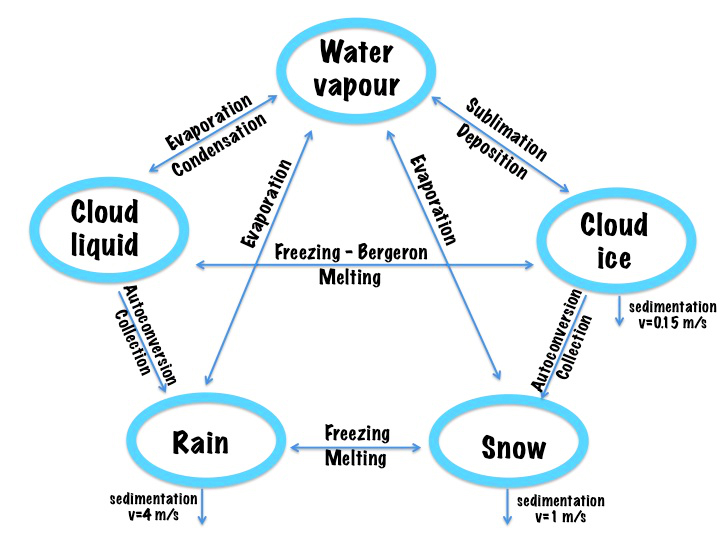
\includegraphics[width=0.6\textwidth]{scheme_var2.jpg}
\end{center}
\caption{\small Schematics of the new scheme, showing the 5 prognostic variables and  how they are related to each other through microphysical processes}
\label{fig:newscheme}
\end{figure}

\paragraph{Temperature tendency.}
The impact on temperature is computed from the conservation of liquid-water
potential temperature $T_L$:

\begin{equation}
  T_L = T - \frac{L_v}{C_p}(q_l + q_r) - \frac{L_s}{C_p}(q_i + q_s)
\end{equation}

Since $dT_L/dt = 0$ in the absence of diabatic forcing, the temperature
tendency is:

\begin{equation}
  \frac{\partial T}{\partial t} = \sum_{x}\frac{L(x)}{C_p}\!\left(
  \frac{dq_x}{dt} - D_{q_x} - \frac{1}{\rho}\frac{\partial}{\partial z}
  (\rho V_x q_x)\right)
\end{equation}

where $L(x)$ is the appropriate latent heat (vaporisation or sublimation),
and $D_{q_x}$ is the convective detrainment rate for species $x$.

\paragraph{Conservation check.}
At the end of each timestep the scheme verifies conservation of total water
and of moist static energy $h = C_p T + gz + L q_x$.  Any residual is
redistributed proportionally to close the budget.

\subsubsection{WRF Single-Moment 5-Class Scheme (WSM5)}
\label{sec:wsm5}

The WSM5 scheme \citep{Hong_04} is a bulk, single-moment microphysics
parameterisation that predicts the mixing ratios of five water species: vapour
$q_v$, cloud water $q_c$, cloud ice $q_i$, rain $q_r$, and snow $q_s$.  It
was developed by \cite{Hong_04} based on earlier work by \cite{Dudhia_89} and
Lin et al., and was ported to RegCM from the WRF model.  All precipitating
species (rain and snow) are assumed to follow inverse-exponential size
distributions with prescribed intercept parameters ($n_{0r} = 8\times10^6$
m$^{-4}$, $n_{0s}$ temperature-dependent), and their terminal velocities scale
with the local air density.  Cloud ice number concentration is diagnosed from
the ice water content rather than prognosed.

The scheme is integrated over each physics timestep using an inner sub-loop
with a maximum sub-step of 120~s.  Within each sub-step, sedimentation of rain
and snow is computed first using a semi-Lagrangian piecewise-linear method
\citep{Juang_10}, followed by the full set of microphysical process rates.

\paragraph{Cold processes.}
Ice nucleation ($q_v \to q_i$) follows a temperature-threshold approach
(Meyers et al.\ 1992 for heterogeneous nucleation below 0°C; homogeneous
freezing below $-$40°C).  Ice deposition and sublimation ($q_v \leftrightarrow
q_i$) are computed from the vapour supersaturation over ice.  Snow deposition
($q_v \to q_s$) and snow autoconversion from ice ($q_i \to q_s$) are included,
as well as collection of cloud ice by snow ($q_i \to q_s$, rate $P_{saci}$)
capped at $q_i/\Delta t$.  Snow melts to rain ($q_s \to q_r$) when $T > 0$°C.

\paragraph{Warm processes.}
Cloud water autoconversion to rain ($q_c \to q_r$) follows a threshold
formulation with a collection efficiency of 0.55 and a critical cloud droplet
radius of $8$~\textmu m.  Collection of cloud water by rain ($q_c \to q_r$,
accretion $P_{racw}$) and below-cloud evaporation of rain ($q_r \to q_v$) are
also included.  Condensation is diagnosed from the saturation adjustment.

\subsubsection{WRF Single-Moment 7-Class Scheme (WSM7)}
\label{sec:wsm7}

The WSM7 scheme \citep{HongLim_06} extends WSM5 by adding graupel and hail as
two additional single-moment precipitating species, giving seven classes in
total: vapour, cloud water, cloud ice, rain, snow, graupel, and hail.  Size
distributions for graupel ($n_{0g} = 4\times10^6$ m$^{-4}$, density
500~kg~m$^{-3}$) and hail ($n_{0h} = 4\times10^4$ m$^{-4}$, density
912~kg~m$^{-3}$) are inverse-exponential.  Terminal velocities for all species
follow power-law fits to the slope parameter of their respective distributions,
with coefficients $(a_g, b_g) = (330.0, 0.8)$ for graupel and
$(a_h, b_h) = (285.0, 0.8)$ for hail.

Additional cold-cloud processes relative to WSM5 include: accretion of rain,
cloud water, and cloud ice by graupel and hail; conversion of snow to graupel
by riming; conversion of graupel to hail by wet growth; and deposition and
sublimation of both graupel and hail.  Wet growth of graupel and hail is
computed from the Bigg (1953) / Musil (1970) wet-growth criterion: when the
latent heat released by riming cannot be shed fast enough, the hydrometeor
surface becomes liquid and growth transitions to the wet-growth rate
$P_{gwet}$ or $P_{hwet}$.  Ice supersaturation is consumed in priority order:
rain evaporation, cloud-ice deposition, snow deposition, graupel deposition,
hail deposition, then ice nucleation.

\subsubsection{WRF Double-Moment 7-Class Scheme (WDM7)}
\label{sec:wdm7}

The WDM7 scheme \citep{LimHong_10} extends WSM7 to a partial double-moment
formulation by adding prognostic number concentrations for cloud condensation
nuclei $N_{CCN}$, cloud droplets $N_c$, and rain $N_r$.  All ice-phase species
(cloud ice, snow, graupel, hail) remain single-moment with prescribed intercept
parameters as in WSM7.  The scheme is the most physically complete
microphysics option in RegCM.

\paragraph{CCN and cloud droplet number.}
The prognostic CCN number concentration $N_{CCN}$ is advected and diffused by
the dynamical core.  When a grid cell is supersaturated over liquid
($RH_l > 1$), a fraction of the available CCN activates into cloud droplets
following the power-law activation spectrum of \cite{KhairoutdinovKogan_00}:

\begin{equation}
  N_{act} = \max\!\left(0,\; (N_{CCN} + N_c)\,
            \min\!\left(1, \left(\frac{RH_l}{RH_{max}}\right)^{k_{act}}\right)
            - N_c\right) \cdot \frac{1}{\Delta t}
\end{equation}

where $k_{act}$ is the activation exponent and $RH_{max}$ is the saturation
cap.  The mass of newly activated droplets $q_{act}$ is diagnosed from an
assumed initial droplet radius of $r_0 = 1$~\textmu m.  $N_{CCN}$ decreases
and $N_c$ increases by $N_{act}\Delta t$ at each sub-step.

\paragraph{Double-moment warm rain.}
The cloud droplet size distribution is assumed to be a gamma distribution
characterised by its number concentration $N_c$ and mixing ratio $q_c$, giving
the slope parameter $\lambda_c = (N_c \pi \rho_w / (6 q_c \rho))^{1/3}$.  The
rain size distribution is inverse-exponential with slope $\lambda_r$ diagnosed
from $N_r$ and $q_r$.  Autoconversion of cloud water to rain follows
\cite{KhairoutdinovKogan_00}:

\begin{equation}
  P_{raut} = K\,q_c^{a}\,N_c^{b},
  \quad
  N_{raut} = 3.5\times10^9\,\rho\,P_{raut}
\end{equation}

Self-collection of rain droplets ($P_{rcol}$), collection of cloud droplets by
rain ($P_{racw}$), and their number counterparts are all computed from the
double-moment distributions, giving rain that is sensitive to both the
aerosol environment (via $N_{CCN}$) and the local drop size spectrum.

\subsection{Ocean flux Parameterization}

\ac{BATS} uses standard Monin-Obukhov similarity relations to compute the
fluxes with no
special treatment of convective and very stable conditions.  In addition, the
roughness length is set to a constant, i.e. it is not a function of wind and
stability.  

The Zeng scheme describes all stability conditions and
includes a gustiness velocity to account for the additional flux induced by
boundary layer scale variability. Sensible heat (${\rm SH}$), latent heat (${\rm
LH}$), and momentum ($\tau$) fluxes between the sea surface and lower atmosphere
are calculated using the following bulk aerodynamic algorithms,
    
\begin{eqnarray}
\tau = \rho_a {u_{\ast}}^2 ({u_{x}}^2 + {u_{y}}^2)^{1/2} / u \\ \nonumber \\
{\rm SH} = -\rho_a C_{pa} u_{\ast} \theta_{\ast} \hspace{.6cm} \\ \nonumber \\
{\rm LH} =  -\rho_a L_{e} u_{\ast} q_{\ast}  \hspace{.65cm}
\end{eqnarray}

where $u_x$ and $u_y$ are mean wind components, $u_{\ast}$ is the
frictional wind velocity, $\theta_{\ast}$ is the temperature scaling parameter,
$q_{\ast}$ is the specific humidity scaling parameter,  $\rho_a$ is air density,
$C_{pa}$ is specific heat of air, and $L_{e}$ is the latent heat of
vaporization.  For further details on the calculation of these parameters refer
to \cite{Zeng_98}.
 
\subsection{Prognostic Sea Surface Skin Temperature Scheme}

By default in \ac{RegCM}, sea surface temperatures (SST) are prescribed every
six hours from temporally interpolated weekly or monthly SST products.
These products, which are produced from satellite retrievals and in-situ
measurements, are representative of the mean temperature in the top
few meters of the ocean. However, the actual SST can differ significantly
from this mean temperature due to the cool-skin and warm-layer effects
described by \cite{Fairall_96}. To improve the calculation of diurnal fluxes
over the ocean, the prognostic SST scheme described by \cite{Zeng_05} was
implemented in \ac{RegCM4}. The scheme is based on a two-layer
one-dimensional heat transfer model, with the top layer representing the
upper few millimeters of the ocean which is cooled by net longwave radiation
loss and surface fluxes. The bottom layer is three meters thick, it is warmer by
solar radiation and exchanges heat with the top layer. This diurnal SST
scheme appears to provide significant, although not major, effects on the
model climatology mostly over tropical oceans, for example the Indian ocean,
and it is now used as default in \ac{RegCM4}.

\subsection{Pressure Gradient Scheme}

Two options are available for
calculating the pressure gradient force.  The normal way uses the full fields.
The other way is the hydrostatic deduction scheme which makes use of a
perturbation temperature.  In this scheme, extra smoothing on the top is done in
order to reduce errors related to the PGF calculation. 

\subsection{Lake Model}
The lake model developed by \cite{Hostetler_93} can
be interactively coupled to the atmospheric model.  In the lake model, fluxes of
heat, moisture, and momentum are calculated based on meteorological inputs and
the lake surface temperature and albedo.  Heat is transferred vertically between
lake model layers by eddy and convective mixing.  Ice and snow may cover part or
all of the lake surface.

In the lake model, the prognostic equation for temperature is

\begin{eqnarray}
{\partial{T}\over \partial{t}} = (k_e + k_m) {\partial^2{T}\over \partial{z}^2 }
\end{eqnarray}

where $T$ is the temperature of the lake layer, and $k_e$ and $k_m$
are the eddy and molecular diffusivities, respectively.   The parameterization
of \cite{Henderson-Sellers_86} is used to calculate $k_e$ and $k_m$ is set to a
constant value of $39 \times 10^{-7}~m^2~s^{-1}$ except under ice and at the
deepest points in the lake.

Sensible and latent heat fluxes from the lake are calculated using  the BATS
parameterizations \cite{Dickinson_93}.  The bulk aerodynamic formulations for
latent heat flux ($F_q$) and sensible heat flux ($F_s$) are as follows,

\begin{eqnarray}
F_q = \rho_a C_D V_a L_v (q_s - q_a) \\ F_s = \rho_a C_p C_D V_a (T_s - T_a)
\end{eqnarray}

where the subscripts $s$ and $a$ refer to surface and air,
respectively; $\rho_a$ is the density of air, $V_a$ is the wind speed, $C_p$
is specific heat at constant pressure, $L_v$ is evaporation latent
heat, $q$ is specific humidity, and $T$ is temperature.  The momentum drag
coefficient, $C_D$, depends on roughness length and the surface bulk Richardson
number.

Under ice-free conditions, the lake surface albedo is calculated as a function
of solar zenith angle \cite{Henderson-Sellers_86}.  Longwave radiation emitted
from the lake is calculated according to the Stefan-Boltzmann law.  The lake
model uses the partial ice cover scheme of \cite{Patterson_88} to represent the
different heat and moisture exchanges between open water and ice surfaces and
the atmosphere, and to calculate the surface energy of lake ice and overlying
snow.  For further details refer to \cite{Hostetler_93} and \cite{Small_99b}. 

\subsection{Aerosols and Dust (Chemistry Model)}

The representation of dust
emission processes is a key element in a dust model and depends on the wind
conditions, the soil characteristics and the particle size. Following
\cite{Marticorena_05} and \cite{Alfaro_01}, here the dust
emission calculation is based on parameterizations of soil aggregate saltation
and sandblasting processes. The main steps in this calculation are: The
specification of soil aggregate size distribution for each model grid cell, the
calculation of a threshold friction velocity leading to erosion and saltation
processes, the calculation of the horizontal saltating soil aggregate mass flux,
and finally the calculation of the vertical transportable dust particle mass
flux generated by the saltating aggregates. In relation to the BATS interface,
these parameterizations become effective in the model for cells dominated by
desert and semi desert land cover. 

% vim: tabstop=8 expandtab shiftwidth=2 softtabstop=2
